% TEMPLATE for Usenix papers, specifically to meet requirements of
%  USENIX '05
% originally a template for producing IEEE-format articles using LaTeX.
%   written by Matthew Ward, CS Department, Worcester Polytechnic Institute.
% adapted by David Beazley for his excellent SWIG paper in Proceedings,
%   Tcl 96
% turned into a smartass generic template by De Clarke, with thanks to
%   both the above pioneers
% use at your own risk.  Complaints to /dev/null.
% make it two column with no page numbering, default is 10 point

% Munged by Fred Douglis <douglis@research.att.com> 10/97 to separate
% the .sty file from the LaTeX source template, so that people can
% more easily include the .sty file into an existing document.  Also
% changed to more closely follow the style guidelines as represented
% by the Word sample file. 

% Note that since 2010, USENIX does not require endnotes. If you want
% foot of page notes, don't include the endnotes package in the 
% usepackage command, below.

% This version uses the latex2e styles, not the very ancient 2.09 stuff.
\documentclass[letterpaper,twocolumn,10pt]{article}

\usepackage{usenix,epsfig,endnotes}

%\usepackage[utf8]{inputenc}
%\usepackage[T1]{fontenc}
%\usepackage{microtype}
%\usepackage{flushend}

%\usepackage{amsmath}
%\usepackage{amssymb}
\usepackage{pifont}

\usepackage{url}
\usepackage{multirow}
\usepackage{listings}
\usepackage{booktabs}
%\usepackage{tikz}
\usepackage{xspace}

\newcommand{\psharp}{P\#\xspace}
\newcommand{\csharp}{C\#\xspace}

\newcommand{\cmark}{\ding{51}}
\newcommand{\xmark}{\ding{55}}

\usepackage{color}
\definecolor{light-gray}{gray}{0.40}
\newcommand{\SQComment}[1]{\textcolor{red}{Shaz: #1}}
\newcommand{\PDComment}[1]{\textcolor{blue}{Pantazis: #1}}
\newcommand{\MMComment}[1]{\textcolor{cyan}{Matt: #1}}
\newcommand{\SCComment}[1]{\textcolor{magenta}{Shuo: #1}}
\newcommand{\CHComment}[1]{\textcolor{blue}{Cheng: #1}}
\newcommand{\PTComment}[1]{\textcolor{light-gray}{Paul: #1}}

\definecolor{bluekeywords}{rgb}{0.13,0.13,1}
\definecolor{greencomments}{rgb}{0,0.5,0}
\definecolor{redstrings}{rgb}{0.9,0,0}

\lstset{language=[Sharp]C,
showspaces=false,
showtabs=false,
breaklines=true,
showstringspaces=false,
breakatwhitespace=true,
escapeinside={(*@}{@*)},
morekeywords={OnEvent, nameof, var, state, cold, hot},
commentstyle=\color{greencomments},
keywordstyle=\color{bluekeywords}\bfseries,
stringstyle=\color{redstrings},
basicstyle=\ttfamily\scriptsize,
columns=fullflexible
}

\begin{document}

%don't want date printed
\date{}

%make title bold and 14 pt font (Latex default is non-bold, 16 pt)
\title{\Large \bf Uncovering Distributed System Bugs during Testing (not Production!)}

%for single author (just remove % characters)
\author{
{\rm Pantazis Deligiannis$^\dagger$, Matt McCutchen$^\diamond$, Paul Thomson$^\dagger$, Shuo Chen$^\star$}\\
{\rm Alastair F. Donaldson$^\dagger$, John Erickson$^\ddagger$, Cheng Huang$^\star$, Akash Lal$^\star$}\\
{\rm Rashmi Mudduluru$^\star$, Shaz Qadeer$^\star$, Wolfram Schulte$^\ddagger$}\\\\
$^\dagger$Imperial College London, $^\ddagger$Microsoft, $^\star$Microsoft Research\\
$^\diamond$Massachusetts Institute of Technology\\
} % end author

\maketitle

% Use the following at camera-ready time to suppress page numbers.
% Comment it out when you first submit the paper for review.
\thispagestyle{empty}


\subsection*{Abstract}
Testing distributed systems is very challenging due to multiple sources of nondeterminism, such as arbitrary interleavings between event handlers and unexpected node failures. Stress testing, commonly used in industry today, is unable to deal with this kind of nondeterminism, which results in the most tricky bugs being missed during testing and only getting exposed in production.

We present a new methodology for systematically testing distributed systems. Our approach involves the use of \psharp, an extension of \csharp that combines a flexible environmental modeling approach with a concurrency testing framework, which can capture and systematically explore all sources of nondeterminism \SCComment{this paper mainly focuses on the nondet due to scheduling, right? There are other sources, e.g., arbitrary input, system call behavior, clock, random number, etc. I feel that ``all sources'' is perhaps an overclaim} \PDComment{We should clarify: as long as you model a source of nondet using \psharp, then you can capture it and control it (not automatically)}. We present two case studies of using \psharp to test production distributed systems inside Microsoft. Using \psharp, we managed to uncover a very subtle bug that was haunting developers for a long time, as they did not have an effective way to reproduce it. \psharp uncovered the bug in a very small setting, which made it easy to examine traces, identify and fix the problem. \PDComment{we now have many bugs in Matt's system too.}

\section{Introduction}
\label{sec:intro}

Distributed systems are notoriously hard to test. This is due to many well-known sources of \emph{nondeterminism}, such as race conditions in the asynchronous interaction between system components, the use of multithreaded code inside a component, unexpected node failures, unreliable communication channels and message losses, and interaction with clients and external services.
%
All these sources of nondeterminism translate into \emph{exponentially} many execution paths that a distributed system might potentially execute. A bug might hide deep inside one of these paths and only manifest under extremely rare corner cases.

Classic techniques that product groups employ to test, verify and validate their systems (such as code reviews, stress testing, fault injection, and chaos testing) are unable to capture and control all the aforementioned sources of nondeterminism, which causes the most tricky backs being missed during testing and only getting exposed after a system has been put in production. Discovering and fixing bugs in production, though, is bad for business as it can cost a lot of money and many dissatisfied customers.

We interviewed engineers from the Microsoft Azure team regarding the top problems in distributed system development, and the unified response was that the most critical problem today is how to improve \emph{testing coverage} to find bugs \emph{before} a system goes in production. The need for better testing techniques is not specific to Microsoft; other companies, such as Amazon and Google, publicly acknowledge~\cite{newcombe2015aws} that testing methodologies have to improve to be able to reason about the correctness of increasingly more complex distributed systems.

Amazon recently published an article~\cite{newcombe2015aws} that describes their use of TLA+~\cite{lamport1994temporal} to detect distributed system bugs and prevent them from reaching production. TLA+ is a powerful specification language for verifying distributed protocols, but it is unable to verify the code that is actually being executed. The implied assumption is that a model of the system will be verified, and then the programmers are responsible to match what was verified with the source code of the real system. Although many design bugs can be caught with this approach, there is \emph{no guarantee} that the real distributed system will be free of bugs.

In this work, our goal is to \emph{test what is being executed}. We present a new methodology for testing legacy distributed systems and uncovering bugs before these systems are released in the wild. We achieve this using \psharp~\cite{deligiannis2015psharp}, an extension of the mainstream language \csharp that provides two key capabilities: (i) a flexible way of modeling the environment using simple language features; and (ii) a systematic concurrency testing framework that is able to capture and take control of all the nondeterminism in a real system (together with its modeled environment) and systematically explore execution paths to discover bugs.

We present two case studies of using \psharp to test production distributed systems for Windows Azure inside Microsoft: a distributed storage management system and a live migration protocol. Using \psharp, we managed to uncover a very subtle bug that was haunting developers for a long time as they did not have an effective way to reproduce the bug and nail down the culprit. \psharp uncovered this bug in a very small setting, which made it easy to examine traces, identify and eventually fix the problem.

To summarize, our contributions are as follows:

\begin{itemize}
\item We present a methodology that allows flexible modeling of the environment of a distributed system using simple language mechanisms.
\item Our infrastructure can test production code written in \csharp, which is a mainstream language.
\item We present two case studies of using \psharp to test production distributed systems, finding bugs that could not be found with traditional testing techniques.
\item ...
\end{itemize}


\section{Motivating Example}
\label{sec:motivation}

Microsoft Azure Storage is a cloud storage system that provides customers the ability to store seemingly limitless amounts of data. It has grown from tens of petabytes in 2010 to exabytes in 2015, with the total number of objects stored well-exceeding 60 trillion~\cite{greenberg2015keynote}.

Azure Storage vNext is the next generation storage system for Microsoft Azure, where the primary design target is to scale the storage capacity by more than 100$\times$. Similar to the current system, vNext employs containers, called \emph{extents}, to store data. Extents are typically several gigabytes each, consisting of many data blocks, and replicated over multiple \emph{Extent Nodes} (ENs). However, in contrast to the current system, which employs a Paxos-based, centralized mapping from extents to ENs, vNext achieves its scalability target by employing a \emph{distributed mapping}. In vNext, extents are divided into partitions, with each partition managed by a light-weight \emph{Extent Manager} (ExtMgr). This partitioning is illustrated in Figure~\ref{fig:vnext}.

\begin{figure}[t]
\centering
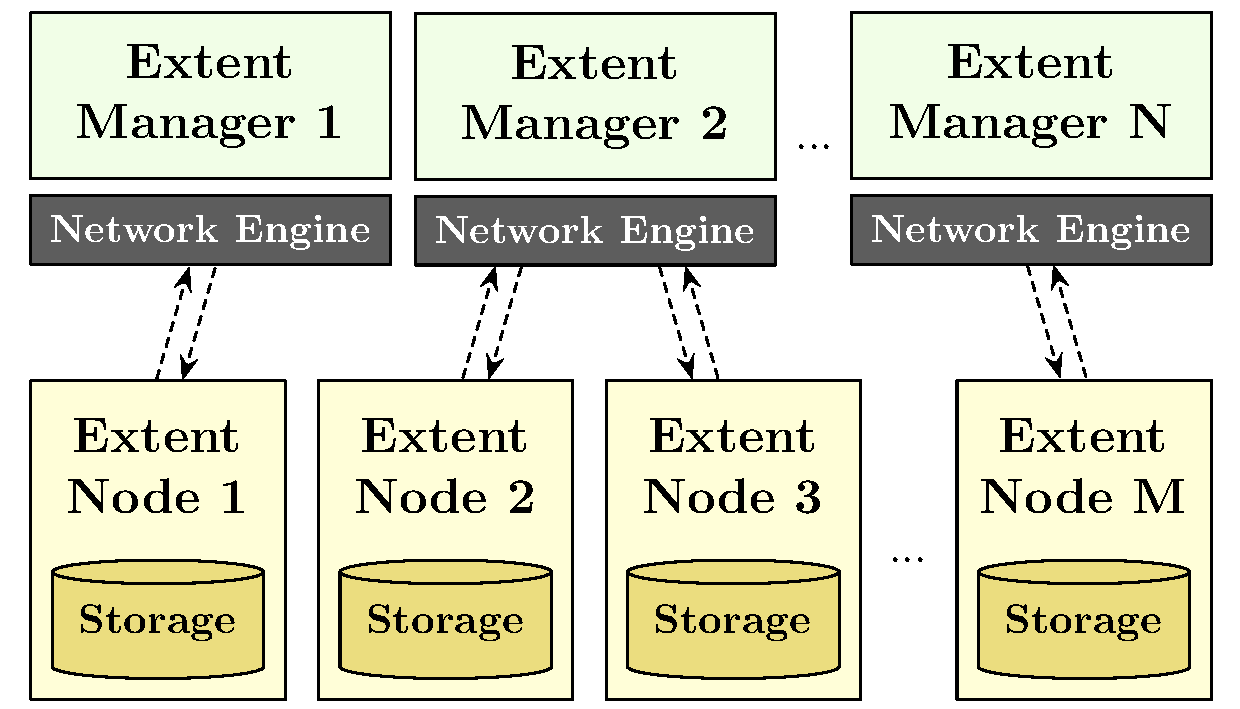
\includegraphics[width=\linewidth]{img/azurestore}
\caption{Top-level components of vNext, a distributed extent management system for Microsoft Azure.}
\label{fig:vnext}
\end{figure}

One of the many responsibilities of an ExtMgr is to ensure that every extent maintains enough \emph{replicas} in the system. To achieve this, an ExtMgr receives frequent periodic \emph{heartbeat} messages from every EN. The failure of an EN is detected by missing heartbeats. An ExtMgr also receives less frequent, but still periodic, \emph{synchronization reports} from every EN. The sync reports list all the extents (and associated metadata) stored on the EN. Based on these two types of messages, an ExtMgr identifies which ENs have failed, and which extents are affected by the failure and are missing replicas as a result. The ExtMgr then schedules tasks to repair the affected extents and distributes the tasks to the necessary ENs. The ENs then repair the extents from their existing replicas in the system and lazily update the ExtMgr via their next periodic sync reports. All this communication between an ExtMgr and the ENs occurs via network engines installed in each component of vNext (see Figure~\ref{fig:vnext}).

To ensure correctness, the developers of vNext have instrumented extensive, multiple levels of testing:
\begin{enumerate}
\item \emph{Unit testing}, in which emulated heartbeats and sync reports are sent to an ExtMgr. These tests check that the messages are processed as expected.

\item \emph{Integration testing}, in which an ExtMgr is launched together with multiple ENs. An EN failure is subsequently injected. These tests check that the affected extents are eventually repaired.

\item \emph{Stress testing}, in which an ExtMgr is launched together with multiple ENs and multiple extents. The test keeps repeating the following process: injecting an EN failure, launching a new EN and checking that the affected extents are eventually repaired.
\end{enumerate}

\noindent
Despite of the extensive testing efforts, the vNext developers have been plagued for months by an elusive bug in the ExtMgr logic. All the unit test suites and integration test suites successfully pass every single time. However, the stress test suite fails \emph{from time to time} after very long executions; in these cases, certain replicas of some extents fail and are never repaired. This bug has proven to be difficult to identify, reproduce and troubleshoot. First, it requires very long executions to trigger. Second, an extent not being repaired is \emph{not} a property that can be easily verified. In practice, the developers rely on a very large time-out period to detect the bug. Finally, by the time that the bug is detected, very long execution traces have been collected, which makes manual inspection tedious and ineffective.

To uncover this bug, as well as many other tricky bugs, the vNext developers are in constant search of a generic and systematic approach for testing production-scale distributed storage systems.

%Since this is a rather typical dilemma in the development of distributed storage systems, a general and systematic approach hopefully would be very helpful to the developers and greatly increase their productivity.


\section{Testing Distributed Systems}
\label{sec:overview}

The goal of our work is to develop testing techniques for detecting and debugging Heisenbugs in distributed storage systems prior to deployment. To achieve our goal, we use \psharp~\cite{deligiannis2015psharp}, an extension of the mainstream \csharp language that provides: (i) language support for \emph{modeling the environment} of distributed systems developed using Microsoft's .NET framework; and (ii) a \emph{testing engine} that can systematically explore all interleavings between asynchronous event handlers, as well as other nondeterministic events such as failures and timeouts.

A \psharp program consists of multiple \emph{state machines} that communicate with each other \emph{asynchronously} by sending and receiving \emph{events}, which may contain an optional \emph{payload}. A \psharp machine declaration is similar to a class declaration in \csharp: it can contain an arbitrary number of fields and methods. However, a machine declaration differs from a class declaration, as it also contains an input event queue, and one or more \emph{states}. Each state can register \emph{actions} to handle incoming events.

\psharp machines run concurrently with each other, each executing an event handling loop that dequeues an event from the input queue and handles it by invoking the registered action. This action might access a field, call a method, transition the machine to a new state, create a new machine, or send an event to another machine. In \psharp, a send operation is \emph{non-blocking}; the event is simply enqueued into the input queue of the target machine, which will dequeue and handle the event concurrently. All this functionality is provided in a lightweight runtime library, built on top of Microsoft's Task Parallel Library~\cite{leijen2009tpl}.

Our approach of using \psharp to test distributed systems, implemented in .NET, requires the developer to perform the following three key modeling tasks. These tasks are illustrated in \S\ref{sec:method} for the Azure Storage vNext system.

\begin{enumerate}
\item
The computation model underlying \psharp is communicating state machines. The environment of the system-under-test must be modeled using the \psharp APIs, while the real components of the system must be wrapped inside \psharp machines. We call this modeled environment the \psharp test harness.

\item
All the asynchrony due to message passing between system components must become explicit and be modeled using the \psharp event-sending APIs. Similarly, all other sources of nondeterminism (e.g. failures and timer expiration) must be modeled using appropriate \psharp APIs. This step allows the \psharp runtime to systematically explore all asynchronous event handler interleavings and all other sources of nondeterminism during testing.

\item
The criteria for correctness of an execution must be specified. Specifications in \psharp can encode either \emph{safety} or \emph{liveness}~\cite{lamport1977proving} properties. Safety specifications generalize the notion of source code assertions; a safety violation is a finite trace leading to an erroneous state. Liveness specifications generalize nontermination; a liveness violation is an infinite trace that exhibits lack of progress.
\end{enumerate}

\noindent
\psharp uses modern object-oriented language features such as \emph{interfaces} and \emph{virtual method dispatch} to connect the real code with the modeled code. Programmers in industry are used to working with such features, and heavily use them in production for testing purposes. In our experience, this significantly lowers the bar for product teams inside Microsoft to embrace \psharp for testing.

In principle, our modeling methodology is \emph{not specific} to \psharp and the .NET framework, and can be used in combination with any other programming framework that has equivalent capabilities. We also argue that our approach is \emph{flexible} since it allows the user to model \emph{as much} or \emph{as little} of the environment as required to achieve the desired level of testing.

\subsection{Specifications}
\label{sec:bg:bugs}

In  this section, we describe how safety and liveness specifications are expressed in \psharp.

\textbf{Safety specifications}.
In addition to the usual assertions for stating safety properties that are local to a machine, \psharp also provides a way to specify global assertions by using a \emph{safety monitor}~\cite{desai2015building}, which is a special machine that can receive, but not send, events.

A safety monitor maintains local state that is modified in response to events received from ordinary (non-monitor) machines. This local state is used to maintain a history of the computation that is relevant to the property being specified. An erroneous global behavior is flagged via an assertion on the private state of the safety monitor. Thus, a \psharp monitor cleanly separates instrumentation state required for specification (inside the monitor) from program state (outside the monitor).

\textbf{Liveness specifications}.
Liveness property specifications are more difficult to encode since they are intended to capture program progress over infinite executions. Violation of a liveness property can only be demonstrated by an infinite execution. Usually, a liveness property is specified via a temporal logic formula~\cite{Pnueli1977,lamport1994temporal}. We take a different approach and allow the programmer to write a \emph{liveness monitor}~\cite{desai2015building}. Similar to a safety monitor, a liveness monitor can receive, but not send, events. Unlike a safety monitor, a liveness monitor contains two types of states: \emph{hot} and \emph{cold}.

A hot state denotes a point in the execution where progress is required but has not happened yet; for example, a node has failed but a new one has not come up yet. A liveness monitor enters a hot state upon receiving notification of an event that requires the system to make progress. The liveness monitor leaves the hot state and enters a cold state upon receiving another event notifying it of progress. An infinite execution is erroneous if the liveness monitor is in a hot state infinitely often but in a cold state only finitely often. Our liveness monitors can encode arbitrary temporal logic properties. A thermometer analogy is useful for understanding liveness monitors: a hot state increases the temperature by a small value; a cold state resets the temperature to zero; a liveness error happens if the temperature becomes infinite.
%The distinction between ordinary and cold states is useful for modeling progress for each instance of an infinite stream of events, such as a periodic request or a periodic timer expiration.

A liveness violation is witnessed by an \emph{infinite} execution in which all concurrently executing \psharp machines are \emph{fairly} scheduled. Unfortunately, it is clearly not possible to generate an infinite execution by executing a program for a finite amount of time. Therefore, our implementation of liveness checking in \psharp approximates an infinite execution using several heuristics. One such heuristic considers an execution longer than a large user-supplied bound as an ``infinite'' execution~\cite{killian2007life, musuvathi2008fair}. Another heuristic maintains a cache of (pieces of) the state of the \psharp program obtained at each step in the execution, and reports an ``infinite'' execution when the latest step results in a cache hit, thus approximating a cycle in the state graph of the program.

%\textbf{Using monitors}.
%To declare a safety or a liveness monitor, the programmer must inherit from the \psharp \texttt{Monitor} class. \psharp monitors are singleton instances and, thus, an ordinary machine does not need a reference to a monitor to send it an event. Instead, an ordinary machine can invoke a monitor by calling \texttt{Monitor<M>(e, p)}, where the parameter \texttt{e} is the event being send, and the parameter \texttt{p} is an optional payload.

\subsection{Systematic testing}
\label{sec:psharp:testing}

The \psharp runtime is a lightweight layer build on top of the Task Parallel Library (TPL) of .NET that implements the semantics of \psharp: creating state machines, executing them concurrently using the default task scheduler of TPL, and sending events and enqueueing them in the appropriate machines. A key capability of the \psharp runtime is that it can execute in \emph{bug-finding} mode, which systematically tests a \psharp program to find bugs using the safety and liveness monitors that were discussed in \S\ref{sec:bg:bugs}.

When the \psharp runtime executes in bug-finding mode, an embedded \emph{systematic concurrency testing engine}~\cite{godefroid1997verisoft, musuvathi2008finding, emmi2011delay} captures and takes control of all sources of non-determinism that are \emph{known} to the \psharp runtime. In particular, the runtime is aware of nondeterminism due to the interleaving of event handlers in different machines. Each send operation to an ordinary (non-monitor) machine, and each create operation of an ordinary machine, creates an interleaving point where the runtime makes a scheduling decision. The runtime is also aware of all nondeterministic events (e.g. failures) that were captured during the modeling process.

The \psharp testing engine will repeatedly execute a program from start to completion, each time exploring a potentially different set of scheduling decisions, until it either reaches a bound (in number of iterations or time), or it hits a property violation. This testing process is fully automatic, has no false-positives (assuming an accurate environment model), and can reproduce found bugs by replaying buggy schedules. After a bug is found, the engine generates a trace that represents the buggy schedule. In contrast to logs typically generated during production, the \psharp trace provides a global order of all communication events and, thus, is easier to debug.

We have implemented two different schedulers inside the \psharp systematic testing engine: a \emph{random} scheduler that makes each nondeterministic choice randomly, and a \emph{probabilistic concurrency testing}~\cite{burckhardt2010pct} (PCT) scheduler. It is straightforward to create a new scheduler by implementing the \texttt{ISchedulingStrategy} interface~\cite{desai2015systematic} exposed by the \psharp libraries. The interface exposes callbacks that are invoked by the \psharp testing engine for taking decisions regarding which machine to schedule next, and can be used for developing both generic and application-specific schedulers.

\textbf{Handling \csharp 5.0 asynchrony}.
The Live Azure Table Migration system (see \S\ref{sec:cases:migration}) heavily uses the \texttt{async} and \texttt{await} \csharp 5.0 language primitives. An \texttt{async} method is able to perform \texttt{await} on a TPL task \emph{without} blocking the current thread. The \csharp compiler achieves this non-blocking behavior by wrapping the code following an \texttt{await} statement in a TPL \emph{task continuation}, and then returning execution to the caller of the \texttt{async} method. The TPL scheduler executes this task continuation when the task being awaited has completed. In principle, this asynchrony can be modeled using the \psharp primitives for machine creation and message passing. However, in our experience, modeling async/await asynchronous code using \psharp is difficult and time consuming, and thus infeasible for large code bases. To tackle this problem, we developed a solution that automatically captures asynchronously created TPL tasks and wraps them in temporary \psharp machines.

Our solution involves using a \emph{custom task scheduler}, during systematic testing with \psharp, instead of the default TPL scheduler. Assuming that the developer does not explicitly change the task scheduler (something extremely uncommon), any TPL tasks spawned in the \psharp program will be scheduled for execution in the \psharp task scheduler. These tasks will be intercepted by our custom task scheduler and wrapped inside a special, available only internally, task-machine. When the \psharp testing engine schedules a task-machine for execution, the corresponding task is unwrapped and executed. This approach works nicely with the \texttt{async} and \texttt{await} \csharp 5.0 primitives: when an \texttt{async} method is called, the asynchronous TPL task will be automatically wrapped in a task-machine and scheduled by \psharp; for \texttt{await}, no special treatment is required since the task continuation will also be automatically wrapped and scheduled accordingly.


\section{Testing Azure Storage vNext with \psharp}
\label{sec:method}

To uncover the elusive extent repair bug in Azure Storage vNext, its developers wrote a testing harness in \psharp. The developers of vNext expected that it was more likely for the bug to occur in the ExtMgr logic, rather than the EN logic. Hence, the testing harness focuses on the real ExtMgr using mocked ENs.

The testing harness consists of the following \psharp machines (as shown in Figure~\ref{fig:azurestoremodel}):
%\begin{enumerate}
\begin{description}
\item[ExtentManager] acts as a thin wrapper machine for the real ExtMgr component in vNext.

\item[ExtentNode] represents a simplified mocked EN.

\item[TestingDriver] communicates with all other machines, relays messages between the \texttt{ExtentManager} and the \texttt{ExtentNode} machines, and is responsible for driving testing scenarios.

\item[RepairMonitor] collects states from all \texttt{ExtentNode} machines in the testing harness and checks desired properties, such as that an extent is replicated or repaired at the expected ENs.
\end{description}

\begin{figure}[t]
\centering
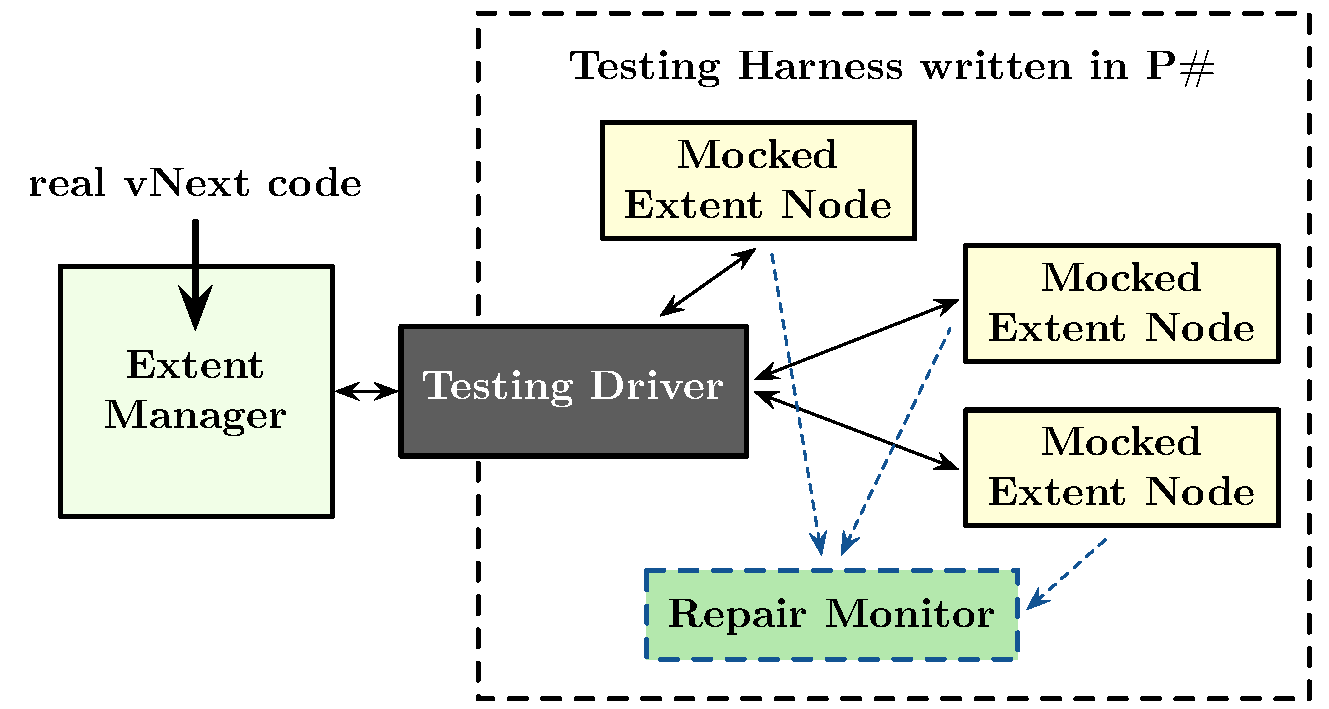
\includegraphics[width=\linewidth]{img/mocked_vnext}
\caption{Real Extent Manager with a mocked environment (each box represents one \psharp machine).}
\label{fig:azurestoremodel}
\end{figure}

\subsection{The ExtentManager machine}
\label{sec:method:wrap_target}

The real ExtMgr in vNext, which is our system-under-test, is wrapped inside the \texttt{ExtentManager} \psharp machine in the testing harness.

\begin{figure*}[t]
\centering
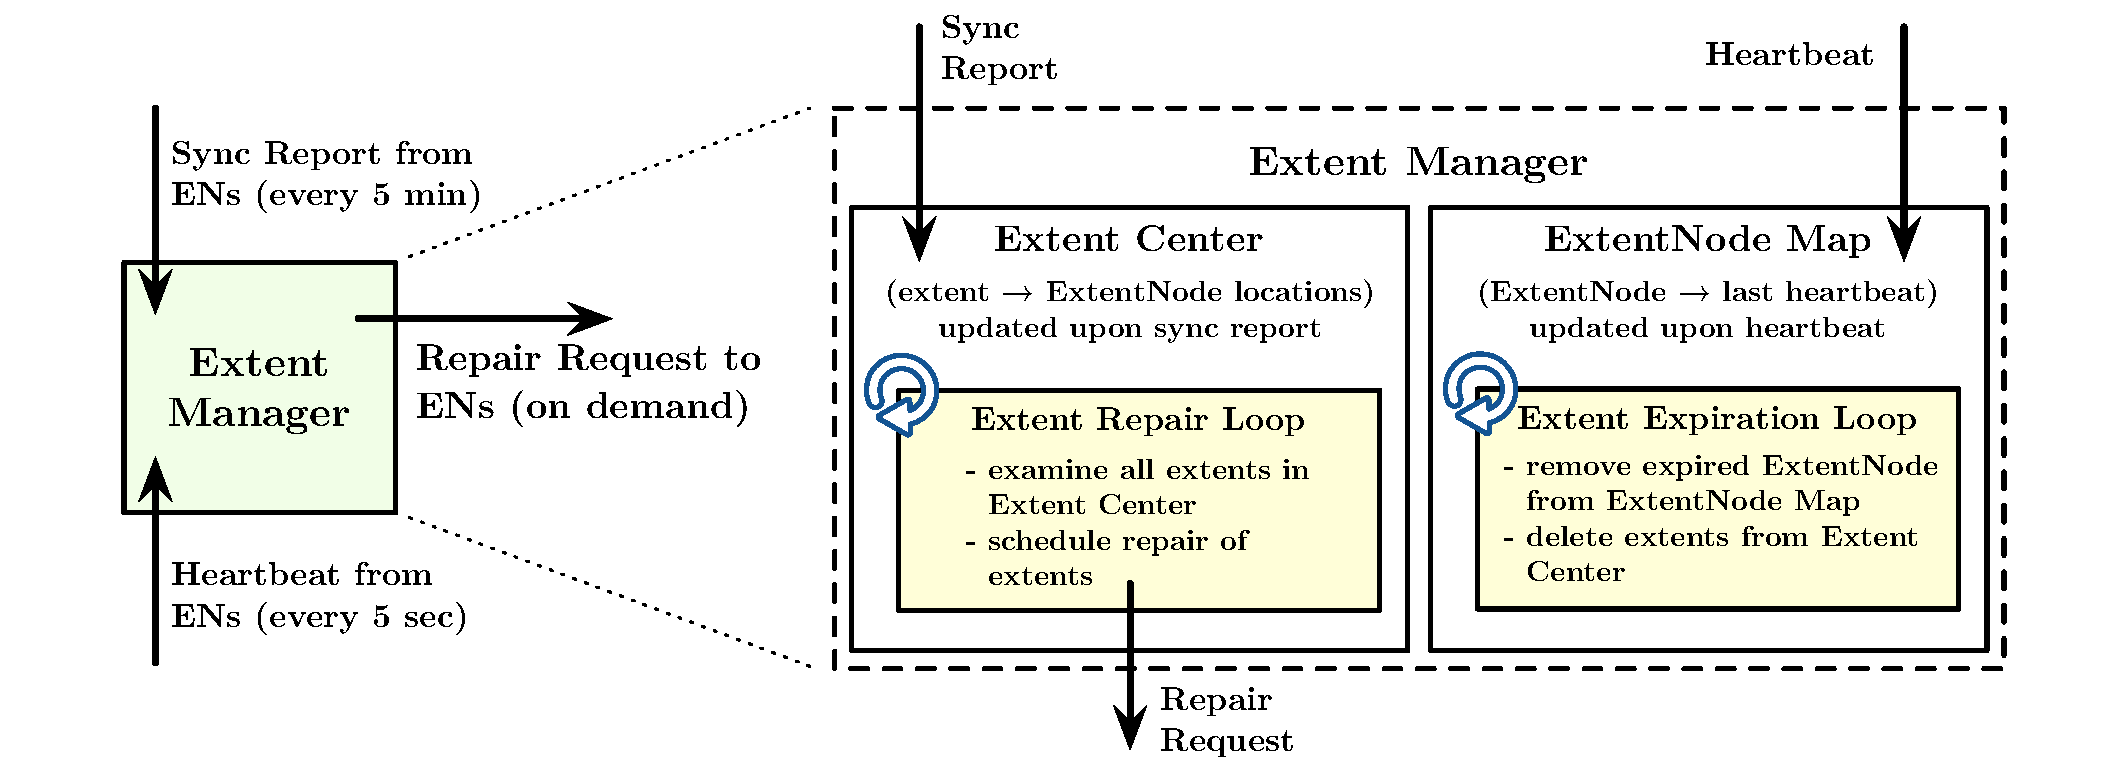
\includegraphics[width=.9\linewidth]{img/extent_manager}
\caption{Internal components of the real Extent Manager in Azure Storage vNext.}
\label{fig:extentmanager}
\end{figure*}

\textbf{Internals of the real Extent Manager}.
Inside the real ExtMgr (see Figure~\ref{fig:extentmanager}), there are two data structures related to extent replication and repair: \texttt{ExtentCenter} and \texttt{ExtentNodeMap}. The \texttt{ExtentCenter} maintains the mapping records from extents to their hosting ENs. It is updated upon the periodic sync reports from the ENs. Recall that the sync report from a particular EN lists all the extents stored at the EN. Its purpose is to update extent manager's possible out-of-date view of the EN with the ground truth. The EN map records the latest heartbeat time from every EN.

The ExtMgr runs internally a periodic {\em EN expiration loop} that is responsible for removing ENs that have been missing heartbeats for an extended period, as well as cleaning up the corresponding records in the \texttt{ExtentCenter}. In addition, the ExtMgr runs a periodic {\em extent repair loop} that examines all the \texttt{ExtentCenter} records, identifies extents with missing replicas, schedules extent repair tasks and sends them to the ENs.

\textbf{Intercepting messages between machines}.
The real ExtMgr uses a network engine to send messages to the ENs. The testing harness mocks the original network engine in vNext and overrides its interface. In this way, the mocked network engine intercepts all outbound messages and relays them to the \texttt{TestingDriver} machine, which is responsible for dispatching the messages to the corresponding \texttt{ExtentNode} machines. As shown in Figure~\ref{fig:enginecode}, the mocked network engine intercepts the outbound messages from the ExtMgr and invokes \texttt{PSharpRuntime.Send(...)} to asynchronously relay the messages to \texttt{TestingDriver}. Conceivably, the mocked network engine could leverage the nondeterminism support in \psharp and choose to drop the messages in a non-deterministic fashion, in case emulating message loss is desirable.

%Method dispatch is the process of selecting which method, from a set of available methods with the same interface, should be invoked during a program's execution. There are two types of method dispatch: \emph{static}, which is resolved during compilation; and \emph{dynamic}, which is resolved in runtime.  \csharp (and thus \psharp) supports both static and dynamic dispatch, and provide the \texttt{virtual} modifier that can be used to declare a method which can be \emph{overridden} during runtime by an inheriting class. This capability is provided by the common language runtime (CLR) of Microsoft's .NET framework, and is a key feature of \csharp as well as other mainstream object-oriented languages.

%Using method dispatch for modeling is straightforward. The system-under-test exposes a set of APIs as \emph{virtual methods}. The developer can then \emph{override} these APIs and replace them with \emph{mocks} that will execute instead of the original implementations during systematic testing with \psharp.

%\begin{figure}[t]
%\begin{lstlisting}
%// Public interface of the real network engine
%class NetworkEngine {
  %public virtual void SendMessage(Socket s, Message msg);
  %public virtual void EnqueueMessage(Message msg);
%}
%
%// The mocked network engine used during testing
%class MockedNetEngine : NetworkEngine {
  %ExtentManager EM; // Handle to actual system-under-test
  %MachineId Env; // Handle to modeled environment
  %
  %public MockedNetEngine(ExtentManager em, MachineId env) {
    %this.EM = em;
    %this.Env = env;
  %}
  %
  %public override void SendMessage(Socket s, Message msg) {
    %PSharpRuntime.Send(this.Env, new MsgEvent(), s, msg);
  %}
  %
  %public override void EnqueueMessage(Message msg) {
    %this.EM.ProcessMessage(msg);
  %}
%}
%\end{lstlisting}
%\vspace{-2mm}
%\caption{The mocked network engine used for testing the Azure Storage vNext system.}
%\label{fig:enginecode}
%%\vspace{-2mm}
%\end{figure}

\begin{figure}[t]
\begin{lstlisting}
// network interface in vNext
class NetworkEngine {
  public virtual void SendMessage(Socket s, Message msg);
}

// mocked engine for intercepting Extent Manager messages
class MockedNetEngine : NetworkEngine {
  public override void SendMessage(Socket s, Message msg) {
    // intercept and relay Extent Manager messages
    PSharpRuntime.Send(this.TestingDriver,
      new MessageFromExtentManagerEvent(), s, msg);
  }
}
\end{lstlisting}
\vspace{-2mm}
\caption{Mocked network engine in vNext.}
\label{fig:enginecode}
%\vspace{-2mm}
\end{figure}

%We now give an example of using dynamic dispatch to model the network engine of an extent manager in the Azure Storage vNext case study (see Figure~\ref{fig:enginecode}). The network engine is responsible for sending to and receiving messages from the various components of the system. During real execution, the network engine uses a custom remote procedure call (RPC) .NET library for communication. For testing, though, it is desirable to replace all calls to this RPC library with \psharp send and receive operations, which can be captured and systematically interleaved to find bugs. We easily achieved this by exposing the original send message operation of the network engine as a virtual method, and then overriding it for testing. In the overridden method, we created a \psharp event and then we wrapped the original message in this event's payload. Then, instead of invoking the RPC library, we invoke the \texttt{PSharpRuntime.Send(...)} method, which asynchronously sends the event (containing the original message) to the target extent node machine.

%For mocking the receive operation, we take advantage of the implicit receive of events in \psharp machines. When a extent node machine receives an event, an appropriate event handler is invoked, which extracts the original message from the payload and then handles it accordingly.

\textbf{Specifics of the ExtentManager machine}.
Figure~\ref{fig:wrap_target} shows code snippets from the \texttt{ExtentManager} \psharp machine. \texttt{ExtentManager} is a thin wrapper of the real ExtMgr. The mocked network engine replaces the real one in ExtMgr, intercepts all the outbound messages from ExtMgr and relays them to \texttt{TestingDriver}.

%A typical wrapper machine contains a handle (as a field) to the system component that is being wrapped (in our case the real Extent Manager object) and the event handlers are responsible for translating any received events to method calls in the real code that is being tested. The \texttt{ExtentManager} is accompanied by a mocked version of the real Network Engine class. The real Extent Manager is communicating with the outside world via remote procedure calls, but in \psharp harness we want to capture this communicating and expose it as calls to \psharp communicating primitives. This is discussed in detail in \S\ref{sec:method:model:dispath}.

%As shown in Figure~\ref{fig:wrap_target}, the \texttt{ExtentManagerMachine} is a wrapper machine and is used to connect the \psharp modeled code with the legacy \csharp code. A typical wrapper machine contains a handle (as a field) to the system component that is being wrapped (in our case the real Extent Manager object) and the event handlers are responsible for translating any received events to method calls in the real code that is being tested. The \texttt{ExtentManager} is accompanied by a mocked version of the real Network Engine class. The real Extent Manager is communicating with the outside world via remote procedure calls, but in \psharp harness we want to capture this communicating and expose it as calls to \psharp communicating primitives. This is discussed in detail in \S\ref{sec:method:model:dispath}.

\begin{figure}[t]
\begin{lstlisting}
// Wrapping the target vNext component in a P# machine
class ExtentManagerMachine : Machine {
  private ExtentManager extMgr; // real vNext code

  void Init() {
    extMgr = new ExtentManager();
    extMgr.netEngine = new MockedNetEngine(); // mock network
    extMgr.isMockingTimer = true;	 // disable internal timer
  }

  [OnEvent(MessageFromExtentNode, DeliverExtentNodeMessage)]
  void DeliverExtentNodeMessage() {
    var msg = (ExtentNodeMessage)this.Payload;
    // relay messages from Extent Node to Extent Manager
    extMgr.ProcessMessage(msg);
  }
	
  [OnEvent(TimerTick), nameof(ProcessExtentRepair))]
  void ProcessExtentRepair() {
    // extent repair loop driven by external timer
    extMgr.ProcessEvent(new ExtentRepairEvent());
  }
}
\end{lstlisting}
\vspace{-2mm}
\caption{System-under-test: instance of the real Extent Manager wrapped inside the \texttt{ExtentManager} machine.}
\label{fig:wrap_target}
%\vspace{-2mm}
\end{figure}

Messages coming from the ENs do \emph{not} go through the mocked network engine. They are delivered to the \texttt{ExtentManager} machine directly and trigger an action that invokes the messages on the internal ExtMgr with \texttt{extMgr.ProcessSingleMessage}. The benefit of this approach is that ExtMgr can be tested without modifying its code; ExtMgr is simply unaware of the testing harness and behaves as if it running in a real distributed environment and communicating with real ENs.

System correctness should \emph{not} hinge on the frequency of any individual timer. Instead, all nondeterminism due to timing-related events must be delegated to \psharp. To achieve this, all timers inside ExtMgr are disabled, and the EN expiration loop and the extent repair loop are driven instead by timers modeled in \psharp, an approach that was used in previous work~\cite{desai2015building}. The \psharp timers send nondeterministic timeout events that are controlled by the \psharp runtime. Hence, the \psharp testing engine has the freedom to schedule arbitrary interleavings between timeout events and all other regular system events.

\subsection{The ExtentNode machine}
\label{sec:method:mock_en}

The \texttt{ExtentNode} machine is a simplified version of the original EN. The machine omits much of the complex details of a real EN, and only mocks the logic necessary for the testing scenarios. This mocked logic includes: repairing an extent from its replica, and sending sync reports and heartbeat messages periodically to the \texttt{ExtentManager} machine.

The testing harness leverages components of Azure Storage vNext whenever it is appropriate. For example, the \texttt{ExtentNode} machine re-uses the \texttt{ExtentCenter} data structure, a component that is used inside a real EN for extent bookkeeping.

In the mocked extent repair logic, \texttt{ExtentNode} takes action upon receiving an extent repair request from the \texttt{ExtentManager} machine. It sends a copy request to a source \texttt{ExtentNode} machine where a replica is stored. After receiving an \texttt{ExtentCopyResponse} event from the source, it updates the internal \texttt{ExtentCenter}, as illustrated in Figure~\ref{fig:mocked_en}. 

In the mocked EN sync logic, the machine is again driven by an external timer provided by \psharp. It prepares a sync report with \texttt{extCtr.GetSyncReport(...)} and asynchronously sends the report to \texttt{ExtentManager} with \texttt{PSharpRuntime.Send(...)}.

%\begin{figure}[t]
%\begin{lstlisting}
%// Wrapping the target vNext component in P#
%class ExtentNodeMachine : Machine {
  %private ExtentNode.ExtentCenter extCtr; // real vNext component
%
	%[OnEventDoAction(typeof(RepairExtentRequestEvent), nameof(ProcessRepairExtentRequest))]
	%[OnEventDoAction(typeof(DownloadExtentRequestEvent), nameof(ProcessDownloadExtentRequestEvent))]
	%[OnEventDoAction(typeof(DownloadExtentResponseEvent), nameof(ProcessDownloadExtentResponseEvent))]
	%[OnEventDoAction(typeof(TimerTickEvent), nameof(ProcessExtentNodeSyncEvent))]
%
  %void ProcessRepairExtentRequest()
  %{
    %var source = GetRepairSourceMachine(this.Payload);
    %PSharpRuntime.Send(source, new DownloadExtentRequestEvent(), this.Payload);
  %}
%
  %void ProcessDownloadExtentRequestEvent()
  %{
	  %var destination = GetRepairDestinationMachine(this.Payload);
    %var ext_id = GetExtentID(this.Payload);
    %
		%Extent ext;
    %if (extCtr.TryGet(ext_id, out ext))
      %PSharpRuntime.Send(destination, new DownloadExtentResponseEvent(), ext);
  %}
%
  %void ProcessDownloadExtentResponseEvent()
  %{
    %var ext = (Extent)this.Payload;
    %extCtr.AddExtent(ext);
%
    %this.Monitor<RepairMonitor>(new NotifyExtentRepairCompletion(), this.NodeID);
  %}
%
  %void ProcessExtentNodeSyncEvent()
  %{
    %var sync = new ExtentNodeSync(this.NodeID);
    %extCtr.Extents.ForEach(ext =>
      %{
        %var rec = new ExtentRecord(ext.ExtentID, ext.Length, ext.Sealed);
        %sync.ExtentRecs.Add(rec);
      %});
    %PSharpRuntime.Send(this.NameNode, new NameNodeMessageEvent(), sync);
  %}
%}
%\end{lstlisting}
%\vspace{-2mm}
%\caption{Mocked Extent Node.}
%\label{fig:mocked_en}
%%\vspace{-2mm}
%\end{figure}

%\begin{figure}[t]
%\begin{lstlisting}
%// Mocking Extent Node in P#
%class ExtentNodeMachine : Machine {
  %// use real vNext component whenever appropriate
  %private ExtentNode.ExtentCenter extCtr;
%
  %[OnEventDoAction(typeof(RepairExtentRequestEvent), nameof(ProcessRepairExtentRequest))]
  %[OnEventDoAction(typeof(TimerTickEvent), nameof(ProcessExtentNodeSync))]
%
  %// extent repair logic
  %void ProcessRepairExtentRequest()
  %{
    %var source = GetRepairSourceMachine(this.Payload);
    %PSharpRuntime.Send(source, new DownloadExtentRequestEvent(), this.Payload);
  %}
  %...
%
  %// extent node sync logic
  %void ProcessExtentNodeSync()
  %{
    %var sync = new ExtentNodeSync(this.NodeID);
    %extCtr.Extents.ForEach(ext =>
      %{
        %sync.ExtentRecords.Add(new ExtentRecord(ext));
      %});
    %PSharpRuntime.Send(this.ExtentManagerMachine, new MessageFromExtentNodeEvent(), sync);
  %}
%}
%\end{lstlisting}
%\vspace{-2mm}
%\caption{Mocked Extent Node.}
%\label{fig:mocked_en}
%%\vspace{-2mm}
%\end{figure}

\begin{figure}[t]
\begin{lstlisting}
// Mocking Extent Node in P#
class ExtentNodeMachine : Machine {
  // leverage real vNext component whenever appropriate
  private ExtentNode.ExtentCenter extCtr;

  // extent repair logic
  ...
  [OnEvent(ExtentCopyResponse, ProcessExtentCopyResponse)]
  void ProcessExtentCopyResponse() {
    // extent copy response from source replica
    if (IsCopySucceeded(this.Payload)) {
      var rec = GetExtentRecord(this.Payload);
      extCtr.AddOrUpdate(rec); // update Extent Center
    }
  }

  // extent node sync logic
  [OnEvent(TimerTick, ProcessExtentNodeSync)]
  void ProcessExtentNodeSync() {
    var sync = extCtr.GetSyncReport(); // prepare sync report
    PSharpRuntime.Send(this.ExtentManagerMachine,
      new MessageFromExtentNodeEvent(), sync);
  }
}
\end{lstlisting}
\vspace{-2mm}
\caption{The mocked EN in vNext.}
\label{fig:mocked_en}
%\vspace{-2mm}
\end{figure}

\subsection{The TestingDriver machine}
\label{sec:method:driver}

The \texttt{TestingDriver} machine drives two testing scenarios. In the first scenario, it launches one \texttt{ExtentManager} and three \texttt{ExtentNode} machines, with a single extent on one of the ENs. It waits for the extent to be replicated at the other ENs. In the second scenario, it fails one of the \texttt{ExtentNode} machines and launches a new one. It waits for the extent to be repaired on the new EN. We omit illustrative code snippets due to space constraints.

\subsection{The RepairMonitor machine}
\label{sec:method:monitor}

The \texttt{RepairMonitor} machine is a \psharp liveness monitor (see \S\ref{sec:bg:bugs}) that transitions between a cold and a hot state. Whenever an extent node fails, \texttt{RepairMonitor} is notified. As soon as the number of extent replicas falls below a specified target (three replicas in the current test harness), \texttt{RepairMonitor} transitions into the hot \emph{repairing} state, where the missing replica is being repaired. Whenever a replica is repaired, the \texttt{RepairMonitor} machine is also notified. It transitions into the cold \emph{repaired} state, when the replica number reaches again the target, as illustrated in Figure~\ref{fig:monitor}.

In the extent repair testing scenarios, \texttt{RepairMonitor} checks that it should {\em always eventually} end up in the cold repaired state. Otherwise, the \texttt{RepairMonitor} machine is stuck in the hot repairing state for {\em infinitely} long. This indicates that the corresponding execution sequence results in an extent replica never being repaired, which is a liveness bug.

\begin{figure}[t]
\begin{lstlisting}
class RepairMonitor : Monitor {
  // true: EN has replica, false: EN has no replica
  private Dictionary<Machine, bool> ExtentNode2Replica;

  // cold state: repaired
  [OnEvent(NotifyEnFailure, ProcessExtentNodeFailure)]
  cold state Repaired {
    void ProcessExtentNodeFailure() {
        var node = GetExtentNode(this.Payload);
        ExtentNode2Replica.Remove(node);
        goto Repairing;
    }
  }

  // hot state: repairing
  [OnEvent(NotifyExtentRepaired, ProcessExtentRepaired)]
  hot state Repairing {
    void ProcessExtentRepaired() {
      var node = GetExtentNode(this.Payload);
      ExtentNode2Replica[node] = true;
      if (ReplicaCount == Harness.REPLICA_COUNT_TARGET)
        goto Repaired;
    }
  }
}
\end{lstlisting}
\vspace{-2mm}
\caption{The RepairMonitor machine.}
\label{fig:monitor}
%\vspace{-2mm}
\end{figure}

\subsection{Liveness Bug in Azure Storage vNext}
\label{sec:method:azurestore}

It took less than ten seconds for the \psharp testing engine to report the first occurrence of a liveness bug in vNext (see \S\ref{sec:eval}). Upon examining the debug trace, the developers of vNext were able to quickly confirm the bug.

However, the original \psharp trace did not include sufficient detail to allow the developers to identify the root cause of the problem. Fortunately, running the test harness took very little time, so the developers were able to quickly iterate and add more refined debug outputs in each iteration. After several iterations, the developers were able to pinpoint the exact culprit and immediately propose a solution for fixing the bug. Once the proposed solution was implemented, the developers ran again the test harness. No bugs were found during 100,000 iterations, a process that required only tens of minutes.

The liveness bug occurs in the second testing scenario, where the \texttt{TestingDriver} fails one of the \texttt{ExtentNode} and launches a new one. The \texttt{RepairMonitor} transitions to the hot repairing state and is stuck in the state for infinitely long.

The following is one particular execution sequence resulting in this liveness bug: (i) EN$_0$ fails and is detected by the EN expiration loop; (ii) EN$_0$ is removed from the EN map; (iii) the extent center is updated and the replica count drops from 3 (which is the target) to 2; (iv) ExtMgr receives a sync report from EN$_0$; (v) the extent center is updated and the replica count increases again from 2 to 3. This is problematic since the replica count is equal to the target, which means that the extent repair loop will never schedule any repair task. At the same time, there are only two \emph{true} replicas in the system, which is one less than the target. This execution sequence leads to one missing replica; repeating this process two more times would result in all replicas missing, but ExtMgr still thinking that all replicas are healthy. In production, such a bug can cause a very serious incident of customer data loss.

The culprit is in (iv), where ExtMgr receives a sync report from EN$_0$ after deleting the EN. This may occur in \psharp due to arbitrary interleaving of events. It may also occur, albeit much less frequently, during stress testing due to messages being delayed in the network. This explains why the bug only occurs from time to time during stress testing and requires long executions to manifest. In contrast, \psharp allows the bug to manifest quickly, the developers to iterate rapidly, the culprit to be identified promptly, and the fix to be tested effectively and thoroughly, all of which have the potential to vastly increase the productivity of distributed storage system development.

%%\subsection{Modeling the environment}
%\subsection{Test Harness}
%\label{sec:method:model}
%
%The environment of a distributed system might consist of other distributed systems and services, clients, operating system timers, as well as libraries for networking or other purposes. To be able to systematically test a distributed system, this environment must be modeled and all the interactions between the environment and the system, as well as all the nondeterminism, must be captured and controlled by the \psharp runtime.
%
%%\subsubsection{Creating a test harness using \psharp}
%\subsubsection{Orchestrating Machines}
%\label{sec:method:model:harness}
%
%\begin{figure}[t]
%\centering
%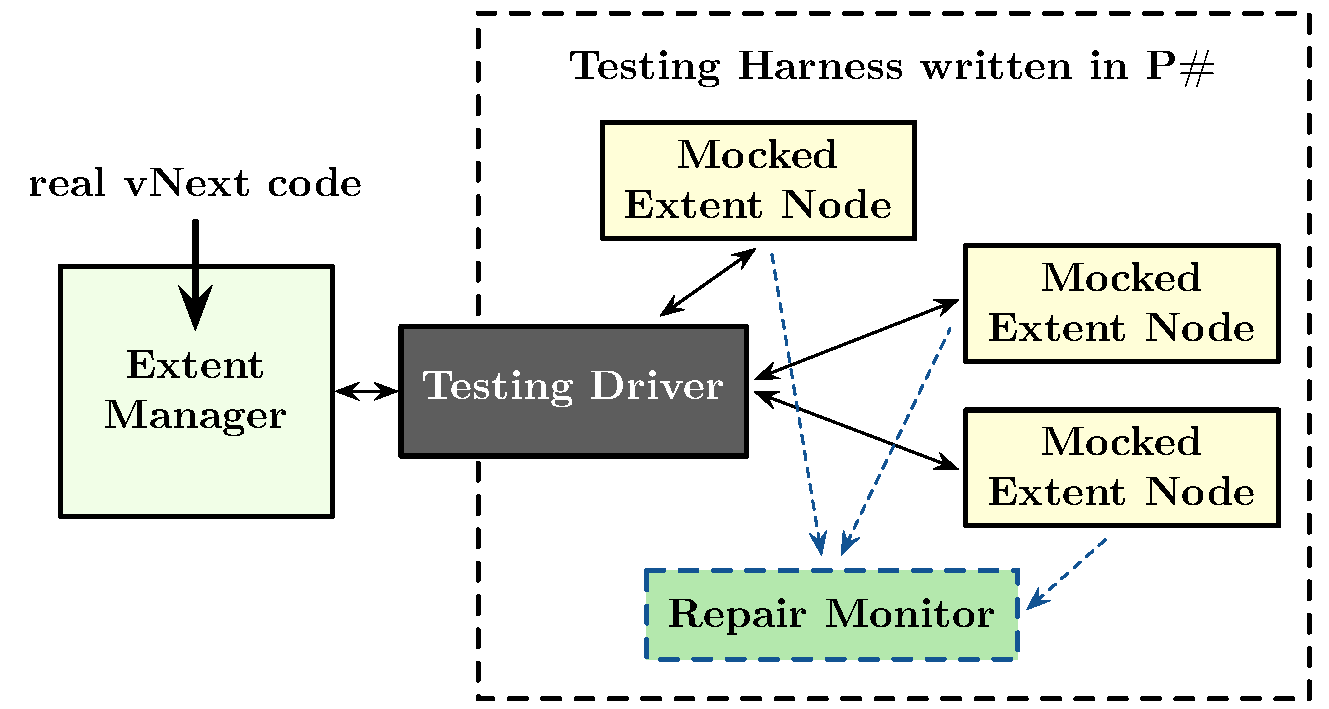
\includegraphics[width=\linewidth]{img/mocked_vnext}
%\caption{The real environment of the Extent Manager is replaced with a mocked version for testing.}
%\label{fig:azurestoremodel}
%\end{figure}
%
%Before being able to use \psharp to test an existing distributed system, the environment of the components that the developer wants to test have to be modeled using the \psharp state machine APIs.  This involves creating mock classes that inherit from the \texttt{Machine} abstract class. The \texttt{Machine} class exposes methods for declaring a state machine (e.g. machine states and state transitions) as well as methods for sending events to other machines, declaring event handlers for received events, and accessing the payload from the latest received event.
%
%In the Azure Storage vNext case study, we created the following \psharp machines: \texttt{Environment}, \texttt{ExtentNode}, \texttt{ExtentManager}, and \texttt{Timer}.
%
%The \texttt{Environment} (denoted with a dashed line box in Figure~\ref{fig:azurestoremodel}) is essentially a ``god'' machine: it is the very first machine that is created; has a handle to all other machines in the harness; and includes the logic based on which the test harness will execute. The programmer is free to create either a finite test harness (e.g. with a predefined number of node failures) or an infinite test harness (e.g. with an unbounded number of failures), as long as any nondeterminism (e.g. when to insert a failure) is captured using the available \psharp APIs.
%
%Finally, the \texttt{Timer} machine models the operating system timer and is responsible for triggering events related to the Azure Storage vNext logic (e.g. synchronization messages, heartbeats and repair logic loops). This is discussed in detail in \S\ref{sec:method:model:timers}.
%
%\subsubsection{Modeling and injecting failures}
%\label{sec:method:model:failures}
%
%In production, each Extent Node of the Azure Storage vNext system periodically (every 5 seconds) sends a heartbeat to the Extent Manager which notifies that the Extent Node is alive. Because we want to model failures and systematically inject them using \psharp, we abstract away the heartbeat mechanism in our harness. However, the Extent Manager logic relies on time intervals to detect node failures (see Figure~\ref{fig:expiration}). The way to abstract this time-related logic and connect the real code with the modeled code is to use virtual dispatch and override the virtual \texttt{IsNodeExpired} method with a mocked version.
%
%\begin{figure}[t]
%\begin{lstlisting}
%// Real code for detecting node expiration
%public virtual bool IsNodeExpired(string id, DateTime time)
%{
  %return DateTime.Compare(time, DateTime.Now) <= 0;
%}
%
%// Mocked code for detecting node expiration
%public override bool IsNodeExpired(string id, DateTime time)
%{
  %return this.DeletedNodes.Contains(id);
%}
%\end{lstlisting}
%\vspace{-2mm}
%\caption{Abstracting the node expiration logic in the Extent Manager component of Azure Storage vNext.}
%\label{fig:expiration}
%%\vspace{-2mm}
%\end{figure}
%
%Figure~\ref{fig:expiration} presents how we mocked the node expiration detection method. Instead of comparing the time interval as in the original code, we now check if the set \texttt{DeletedNodes} contains the id of the Extent Node that we are checking for expiration. If it contains the id, then it means that the node has failed. The \texttt{Environment} machine that we have created as part of our testing \psharp harness, will nondeterministically choose a node to kill, then send the id of this killed node to the Extent Manager wrapper machine, who will in turn add it to the \texttt{DeletedNodes} set.
%
%\subsubsection{Entry point to a \psharp test harness}
%\label{sec:method:model:entrypoint}
%
%A developer can specify the entry point of a \psharp test harness similar to how unit tests are typically written. Figure~\ref{fig:entrypoint} shows the source code of the entry point for the Azure Storage vNext \psharp test harness. The programmer can declare an entry point method using the \texttt{Microsoft.PSharp.Test} attribute. When the \psharp systematic testing engine is invoked, it will scan the binary and attempt to find a static method declared with this attribute. When such a method is found (in our example the \texttt{Execute()} method), the testing engine will invoke it and start testing the program. The systematic engine can optionally run multiple iterations of the test harness, each one potentially exploring a different schedule. In each iteration, the program state will be reset (any static fields must be explicitly reset by the programmer) and the entry point will be re-invoked.
%
%\begin{figure}[t]
%\begin{lstlisting}
%[Microsoft.PSharp.Test]
%public static void Execute()
%{
  %PSharpRuntime.CreateMachine(typeof(Environment));
%}
%\end{lstlisting}
%\vspace{-2mm}
%\caption{Static \csharp method acting as the entry point to the Azure Storage vNext \psharp test harness.}
%\label{fig:entrypoint}
%%\vspace{-2mm}
%\end{figure}
%
%\subsubsection{Abstracting timers}
%\label{sec:method:model:timers}
%
%Distributed systems are often using timers to determine when an event should be send from one component to another. For example, in the Azure Storage vNext system, each Extent Node is associated with a timer that fires of a synchronization message every 5 minutes and a heartbeat every 5 seconds. This timer is related to the liveness bug that we discovered: the synchronization message that gets fired every 5 minutes can potentially race with an Extent Node failure; if it arrives after the node failed, then the bug would manifest. Traditional testing techniques cannot easily find such a bug, due to the very infrequent occurrence of this race due to the timer. 
%
%Our methodology in \psharp to systematically test distributed systems that rely on timers, is to abstract timers away, model them using message passing communication and introduce nondeterminism in their firing. This nondeterminism is introduced using the \psharp \texttt{Nondet()} method, which returns a nondeterministic boolean value that is controlled by the \psharp runtime during systematic testing.
%
%Figure~\ref{fig:timer} shows how we modeled a generic timer in the Azure Storage vNext case study. The Extend Manager, as well as each Extent Node in the harness, is associated with a unique \texttt{Timer} machine. When creating this machine, we pass as a payload the id of the machine that owns this timer. When the \texttt{Timer} machine is created, it stores this id in the \texttt{Owner} field and then transitions to the \texttt{Active} state. In this state, the \texttt{Timer} loops infinitely and nondeterministically (using \texttt{Nondet()}) sends a \texttt{TimerTickEvent} to \texttt{this.Owner}. When the Extent Node owner receives this event, it handles it by generating a synchronization message that is being send to the Extent Manager. Similarly, when the Extent Manager receives a \texttt{TimerTickEvent} from its own \texttt{Timer}, it handles it by nondeterministically invoking repair-related methods in the Extent Repair Center data structure. 
%
%\begin{figure}[t]
%\begin{lstlisting}
%internal class Timer : Machine
%{
  %MachineId Owner; // Id of the owner machine
%
  %[Start]
  %[OnEntry(nameof(InitOnEntryAction))]
  %[OnEventGotoState(typeof(Unit), typeof(Active))]
  %class Init : MachineState { }
%
  %void InitOnEntryAction()
  %{
    %this.Owner = (MachineId)this.Payload;
    %// triggers state transition to Active
    %this.Raise(new Unit());
  %}
%
  %[OnEntry(nameof(ProcessTickEvent))]
  %[OnEventGotoState(typeof(Unit), typeof(Active))]
  %class Active : MachineState { }
%
  %void ProcessTickEvent()
  %{
    %// Nondeterministic boolean choice controlled by P#
    %if (this.Nondet())
      %// sends a timer tick event to the owner machine
      %this.Send(this.Owner, new TimerTickEvent());
    %// triggers state transition to Active
    %this.Raise(new Unit());
  %}
%}
%\end{lstlisting}
%\vspace{-2mm}
%\caption{Timers in Azure Storage vNext are modeled as nondeterministic \psharp machines.}
%\label{fig:timer}
%%\vspace{-2mm}
%\end{figure}


\section{The \psharp Systematic Testing Engine}
\label{sec:psharp}

\subsection{Overview}
\label{sec:psharp:overview}

Draft

\subsection{Liveness checking}
\label{sec:psharp:liveness}

Draft

\subsection{Handling intra-machine concurrency}
\label{sec:psharp:async}

Async/Await

custom schedulers, etc

\subsection{Other}
\label{sec:psharp:other}

Logs/traces -> user can extend them?

\PDComment{mention dependency injection pattern?}


\section{Experience Report}
\label{sec:exp}

The modeling and testing approach described in the earlier sections of the paper is not specific to the vNext system. \psharp is a generic framework for .NET distributed systems. We showcase this capability by presenting developer experience of using \psharp to model and test two other systems used in production inside \Microsoft.

\subsection{Live Table Migration}
%\subsection{Live \Azure Table Migration}
\label{sec:cases:migration}

The Live Table Migration library (MigratingTable) is designed to \emph{transparently} migrate a data set between tables in a
%The Live \Azure Table Migration library (MigratingTable) is designed to \emph{transparently} migrate a data set between tables in an
\Azure Storage service \emph{while} an application is accessing this data set. This case study is particularly interesting because its developers \emph{co-developed} the system with its \psharp test harness to increase confidence in the system. Indeed, this co-development process resulted in the discovery of several tricky bugs before the system went into production (see \S\ref{sec:eval}). The MigratingTable testing effort differs from the vNext case study: the vNext developers focused on specifying a single liveness property, while the MigratingTable test checks complete compliance with an interface (safety) specification.

\textbf{Specifics of the system}.
MigratingTable provides a \emph{virtual table} that has an interface similar to an ordinary \Azure table. This interface is named \texttt{IChainTable}. A virtual table is backed by a pair of \emph{old} and \emph{new} \emph{backend} tables, both of which implement \texttt{IChainTable}. A \emph{migrator} job is responsible for moving all data from the old table to the new table in the background. Meanwhile, each read and write operation issued to the virtual table is translated to a sequence of reads and writes on the backend tables according to a protocol, which intends to guarantee that when multiple applications issue \emph{input} operations to virtual tables that are backed by the same backend tables, the output is compliant with the specification of \texttt{IChainTable} for the combined \emph{input history} as if all the operations were done on a single table. The goal of using \psharp was to systematically test this property.

\begin{figure}[t]
\centering
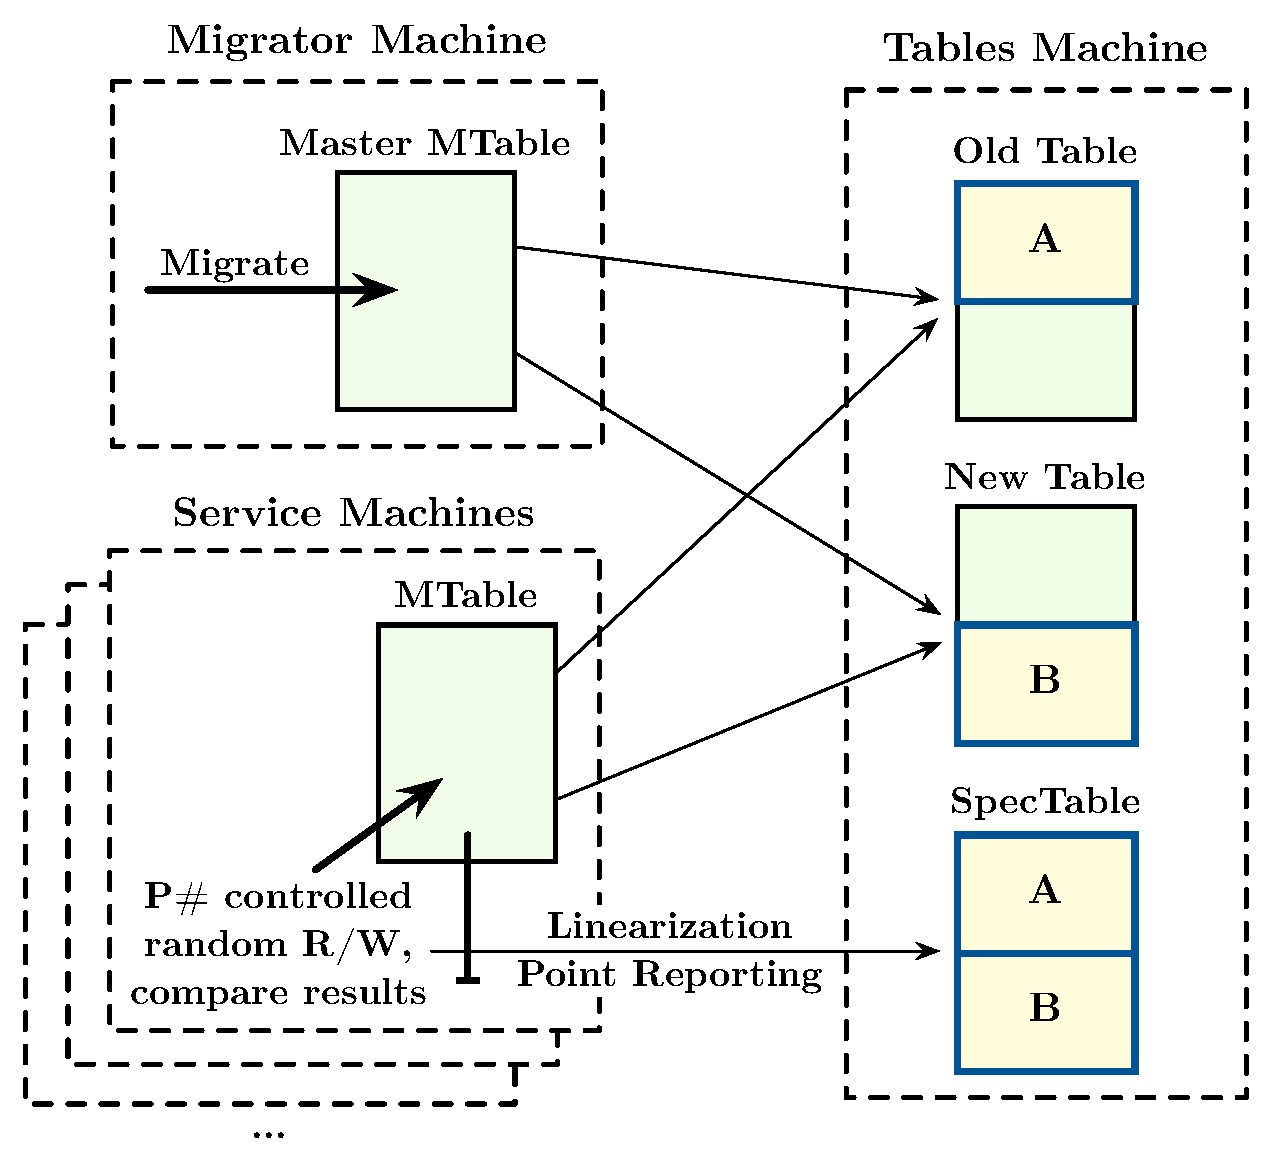
\includegraphics[width=\linewidth]{img/mocked_migration}
\caption{Environment model of MigratingTable (each box with a dotted line represents one \psharp machine).}
\label{fig:mockedmigration}
\end{figure}

\textbf{Testing challenges}.
There are two main challenges behind testing MigratingTable: the system is highly concurrent; and there are many possible input histories. The developers could have chosen specific input histories to test, but they were not confident that this approach would be effective in catching bugs, especially because concurrency increases the potential for difficult-to-foresee interactions between seemingly independent parts of the code. Instead, the developers wrote an in-memory reference implementation of the \texttt{IChainTable} specification, called \texttt{SpecTable}, to which the MigratingTable output on an arbitrary input history can be compared.

\textbf{Modeling and testing with \psharp}.
Figure~\ref{fig:mockedmigration} illustrates the \psharp test harness of MigratingTable. The test harness consists of a collection of \texttt{Service} machines that contain identically configured instances of MigratingTable; a \texttt{Tables} machine, which contains the old and new tables, and an instance of \texttt{SpecTable}; and a \texttt{Migrator} machine that performs the background migration. Each \texttt{Service} machine issues a random sequence of input operations to its MigratingTable, which then sends these operations to the \texttt{Tables} machine.

The developers instrumented MigratingTable to report the intended \emph{linearization point} of each input operation on its corresponding virtual table. This allows the \psharp test harness to keep \texttt{SpecTable} in sync with the virtual table: the \texttt{Service} machine sends each input operation to \texttt{SpecTable} when the linearization point on the virtual table is reached. The output of the operation on the virtual table is then checked against its output on \texttt{SpecTable}.

The \psharp test harness \emph{samples from a distribution} that was defined over all possible input histories within certain bounds, so that under the \emph{small scope hypothesis} that any given bug in MigratingTable leads to incorrect output for at least one input history in the distribution, each iteration of the \psharp systematic testing engine would have a positive probability of detecting the bug.

\psharp captures and controls all the interleaving in the system, and systematically explores them. To ensure that \texttt{SpecTable} is never observed to be out of sync with the backend tables, which could lead to false positives, after the \texttt{Tables} machine processes a backend operation, it enters a state that defers further backend operations until MigratingTable has reported whether the backend operation was a linearization point and (if so) the operation on \texttt{SpecTable} has been completed.

%\begin{figure}[t]
%\centering
%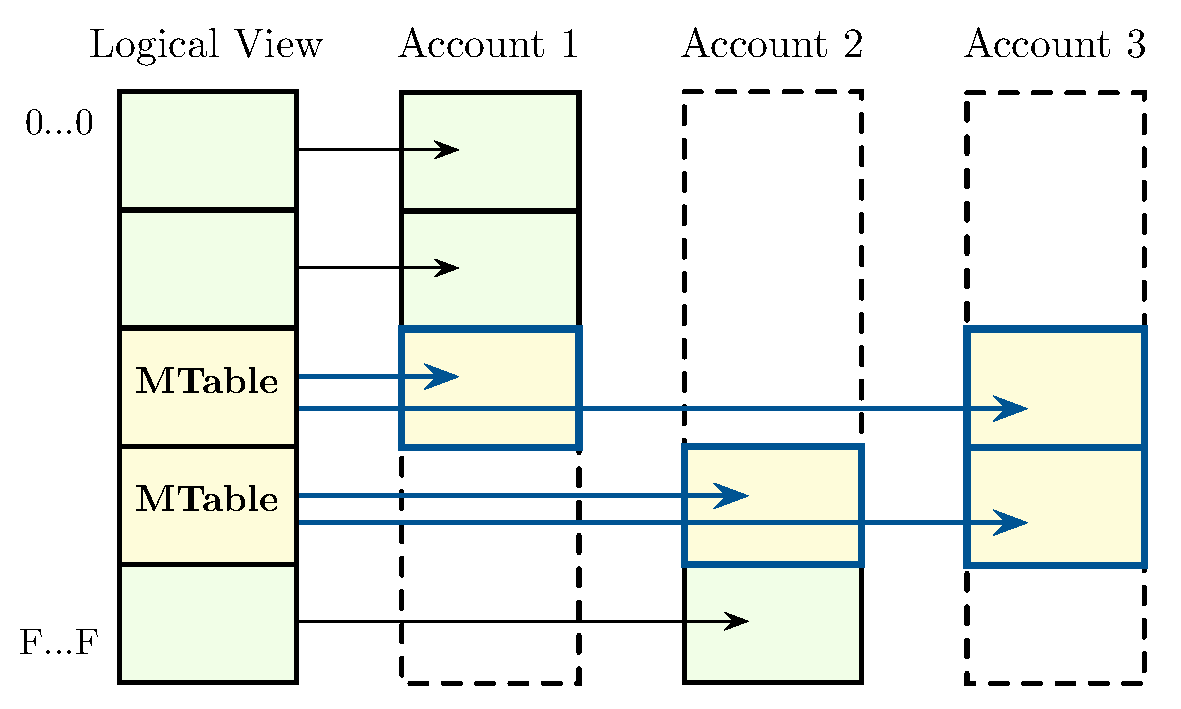
\includegraphics[width=\linewidth]{img/livemigration}
%\caption{Resharding a data set when a third Azure storage account is added. Two key ranges are each migrated to the new account using a MigratingTable instance (abbreviated MTable).}
%\label{fig:livemigration}
%\end{figure}

% N.B. Artifact Services is mentioned at http://research.microsoft.com/en-us/people/schulte/.  Hopefully it's OK to reveal that it was the system in this case study. ~ Matt 2015-08-17
%The initial motivation for MigratingTable was to solve a scaling problem for Artifact Services, an internal Microsoft system with a data set that is sharded across tables in different Azure storage accounts because it exceeds the limit on traffic supported by a single Azure storage account.  As the traffic continues to grow over time, the system needs to reshard the data set across a greater number of Azure storage accounts without interrupting service.  During such a resharding, our sharding manager will identify each key range that should migrate to a different table, and we will use a separate MigratingTable instance for each such key range to actually perform the migration (Figure~\ref{fig:livemigration}).  MigratingTable may also be useful to migrate data to a table with different values of configuration parameters that Azure does not support changing on an existing table, such as geographic location.

%Since we were designing a new concurrent protocol that we expected to become increasingly complex over time as we add optimizations, we planned from the beginning to maintain a \psharp test harness along with the protocol to maintain confidence in its correctness.

%MigratingTable implements an interface called \texttt{IChainTable}, which provides the core read and write functionality of the original Azure table API with one exception: it provides \emph{streaming reads} with a weaker consistency property than multi-page reads in the original API, since the original property would have been difficult to achieve for no benefit to applications we could foresee.  MigratingTable requires that its backend tables also implement \texttt{IChainTable}, and we wrote a simple adapter to expose physical Azure tables as \texttt{IChainTable}.

% N.B. \texttt{SpecTable} = InMemoryTableWithHistory in the current codebase. ~ Matt 2015-08-17

%\psharp takes control of the choice of input history, as well as the schedule, so both can be reproduced using a single random seed. Then, under the \emph{small scope hypothesis} that any bug in MigratingTable leads to incorrect output for at least one input history in our distribution, we have a positive probability of detecting this incorrect output on each iteration of the \psharp test.

%If we had no formalization of the specification and had to rely on expected outputs worked out by hand, this might be the best we could do.  However, since the \texttt{IChainTable} specification is relatively simple and is almost deterministic under sequential calls, it was straightforward to write an in-memory reference implementation called \texttt{SpecTable} to which we can compare the output of MigratingTable on an arbitrary input history.  This gave us the attractive option to sample from a distribution we defined over all possible input histories within certain bounds.

%It was convenient to let \psharp control the choice of input history as well as the schedule so we could reproduce both using a single random seed.  Then, under the \emph{small scope hypothesis} that any bug in MigratingTable leads to incorrect output for at least one input history in our distribution, we have a positive probability of detecting this incorrect output on each iteration of the \psharp test.

%All of our input histories include two application processes.  Each process performs either a single streaming read or a sequence of two atomic calls, each a read or a batch write.  Each batch write call includes one or two operations, where the operation type is chosen from the set supported by \texttt{IChainTable} (Insert, Replace, Merge, Delete, InsertOrReplace, InsertOrMerge, DeleteIfExists) and the row key is chosen from $\{0, \ldots, 5\}$.  If the operation requires an If-Match value, it is equally likely to be \texttt{*}, the current ETag of the row (if it exists), or some non-matching value.  Finally, the new entity includes a user-defined property \texttt{isHappy} whose value is equally likely to be true or false.  For both atomic and streaming reads, the filter expression is equally likely to be empty (i.e., match everything), \texttt{isHappy eq true}, or \texttt{isHappy eq false}.

%As mentioned above, the \texttt{IChainTable} specification is almost deterministic under sequential calls; the only nondeterminism is in the results of streaming reads.  Given a streaming read, \texttt{SpecTable} can compute the set of all results that are compliant with the specification, so we can simply check if the result of MigratingTable is in this set.

%To test MigratingTable, we must supply it with backing tables.  We use \texttt{SpecTable} for this purpose as well, with \psharp choosing the actual result of each streaming read from the valid set.  Our correctness property is then:
% Convert to some theorem-like environment? ~ Matt
%\begin{quote}
%For every execution trace of a collection of MigratingTables backed by the same pair of \emph{old} and \emph{new} \texttt{SpecTable}s in parallel with the migrator job, there exists a linearization of the combined input history such that the output in the original trace matches the output of a ``reference'' \texttt{SpecTable} on the linearized input.
%\end{quote}
%

%The MigratingTable was instrumented to report the intended \emph{linearization point} of each input call, which in our setting is always one of the corresponding \emph{backend calls} to the backend tables (often the last).  Specifically, after each backend call completes, MigratingTable reports whether that call was the linearization point, which may depend on the result of the call.  This makes it possible to check the correctness property as the model executes.

%We use the \psharp random scheduling strategy; we were afraid that an exhaustive strategy would only be feasible within bounds so low that we would miss some bugs.

%We wanted to implement the core MigratingTable algorithms in \csharp ``async/await'' code, like most of Artifact Services, to achieve both good readability and good performance.  We used a method similar to that described in \S\ref{sec:psharp:async} to bring the generated TPL tasks under the control of the \psharp scheduler.  Then we implemented an ``async'' RPC mechanism based on the .NET RealProxy class that automates the generation of proxies for objects hosted by other \psharp machines (in our setting, the service machines use proxies for the \texttt{SpecTable}s and various auxiliary objects hosted by the tables machine).  When a machine calls a method on a proxy, the proxy sends a \psharp message to the host machine, causing it to execute the method call on the original object and send back the result, which the proxy then returns.  Thus, the use of these proxies as \texttt{IChainTable} backends is transparent to the MigratingTable library, thanks to dynamic dispatch.

\subsection{\Azure Service Fabric}
\label{sec:cases:fabric}

\Azure Service Fabric
%\footnote{\url{azure.microsoft.com/campaigns/service-fabric/}}
(or Fabric for short) is a platform and API for creating reliable services that execute on a cluster of machines. 
%The developer writes a service that receives requests (e.g.\ from some client program via HTTP requests) and mutates its state based on these requests. 
In order to make the user-written service \emph{reliable}, Fabric launches several \emph{replicas} (copies) of the service, where each replica runs as a separate process on a different node in the cluster.
%\PTComment{Cut: description of primary and secondaries, and electing a new primary.}
One replica is selected to be the \emph{primary} which serves client requests; the rest are \emph{secondaries}. The primary replicates state changes to the secondaries 
%by sending them \emph{replication requests}.
so that all replicas eventually have the same state. 
If the primary fails,
% (e.g.\ if the node on which the primary is running crashes), 
Fabric elects one of the secondaries to be the new primary and launches another secondary; the new secondary will receive 
%a full or partial copy (depending on whether persistent storage is used) 
a copy
of the state of the new primary in order to ``catch up'' with the other secondaries. 
%Fabric provides a name-resolution service so that clients can always find the current primary.
%The state of the service is replicated from the \emph{primary} replica to the other \emph{secondary} replicas for redundancy.
User-written Fabric services are complex asynchronous and distributed applications, and are thus challenging to test.
% They are interesting targets for systematic testing with \psharp{}.

Our primary goal was to create a \psharp{} model of Fabric to allow
thorough testing of services, where Fabric's asynchrony is controlled 
by the \psharp{} runtime.
The model is written once
to include all behaviours of Fabric, including simulating failures and recovery,
so that it can be reused repeatedly to test multiple Fabric services.
This was the largest modeling exercise among the case studies but the cost
was amortized across testing multiple servies. This is analogous to the work
on driver verification \cite{ball2011slam} where the cost of developing a model
of the Windows kernel was amortized across testing multiple device drivers.
Note that we model the lowest Fabric API layer (\texttt{Fabric.dll})
which is currently not documented for use externally.
We target internally-developed services that invoke the lowest layer. 

\psharp's systematic testing was very helpful in debugging the model itself.
% Without systematic testing, we feel even catching bugs in the model 
% would have been difficult.
In order to perform systematic testing on our model,
we wrote a simple service in \psharp{}
that runs on our Fabric model.
%made up of a single machine
% and executed it on the Fabric model,
% thus yielding a pure \psharp{} system.
We tested a scenario where the primary replica
fails at some non-deterministic point
within the execution.
One such bug that we found
involved
the primary replica
failing
when a secondary replica
was about to receive a copy of the state;
the secondary was then elected to be the new primary
and yet, because the secondary stopped waiting for
a copy of the state, it was
also promoted to be an \emph{active} secondary
(one that has caught up with the other secondaries).
This caused an assertion failure in our model
allowing us to detect and fix this incorrect behaviour.


%\PTComment{Cut: prior work created a Fabric model\ldots}
% Prior work~\cite{deligiannis2015psharp}
% created a model of Fabric with limited functionality;
% it used a mixture of \csharp{} and \psharp{} internally,
% only supported one in-flight replication request
% (which restricts the asynchrony that can be tested),
% and only supported one Fabric service.
% Our new Fabric model was re-written to use only \psharp{}
% internally,
% support an arbitrary number of Fabric services and in-flight replication requests,
% and in general be a more complete model of Fabric.
% Note that \csharp{} code is still required to interface with the existing
% \csharp{} service code.
% We refer to our \csharp{} code
% as the \emph{translation layer}
% and
%  the user-written \csharp{} service code as \emph{user code}. 

%\PTComment{Cut: Figure of model.}
% \begin{figure}[thb]
% \centering
% 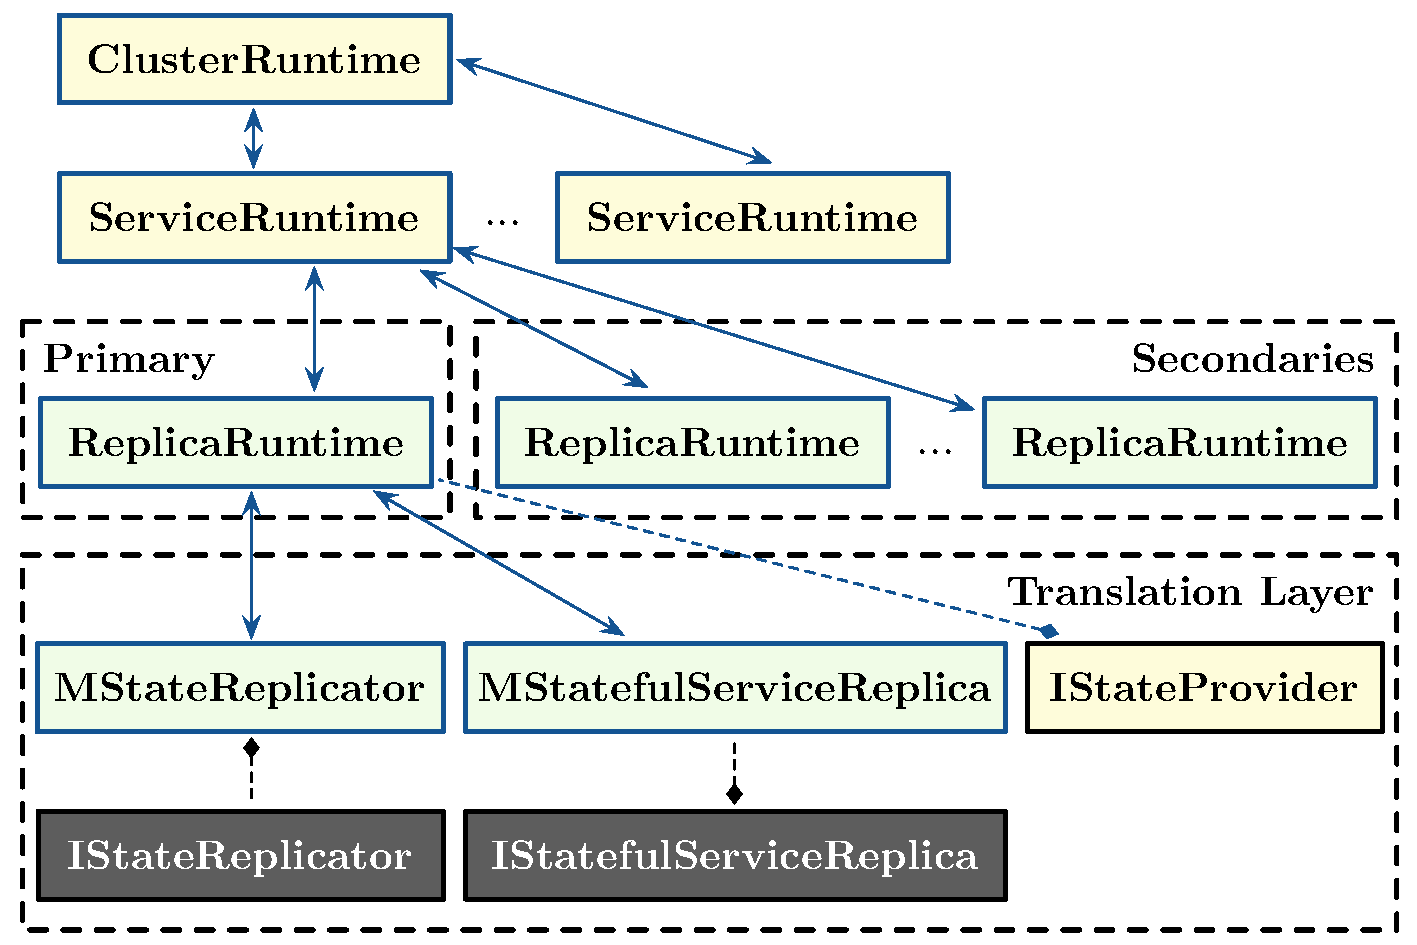
\includegraphics[width=\linewidth]{img/fabricmodel}
% \caption{Overview of the key machines and interfaces in our Fabric model.}
% \label{fig:fabric_model}
% \end{figure}

%\PTComment{Cut: overview of model.}
% An overview of our Fabric model is shown in Figure~\ref{fig:fabric_model}.
% The \texttt{ClusterRuntime} machine 
% handles the creation and management of 
% one or more Fabric services,
% as well as service resolution requests
% which allows for client-service and inter-service communication
% within the model.
% Each Fabric service instance is managed by a \texttt{ServiceRuntime}
% machine, which in turn manages 
% several \texttt{ReplicaRuntime} machines.
% Each \texttt{ReplicaRuntime} communicates with the user code
% via several machines and interfaces from the translation layer
% (only the translation layer for the primary is shown,
% but every \texttt{ReplicaRuntime} has its own instance of the translation layer).
% Note that communication between machines is hierachical;
% thus, communication between \texttt{ReplicaRuntime}s
% (such as the sending of replication requests)
% is via the \texttt{ServiceRuntime} machine for that service.
% This approach does not necessarily reflect how Fabric works in practice.
% Instead, we chose an architecture
% that keeps the model simple
% while still allowing (what we believe to be) realistic
% asynchrony and failure scenarios.

%\PTComment{Cut: Description of how replication works in the model, including how we modeled at a fine granularity.}
% \textbf{Replication example:} In order to replicate a state-mutating operation,
% user code at the primary replica 
% calls \texttt{IStateReplicator.ReplicateAsync},
% passing the serialized operation
% object.
% The operation is sent to the \texttt{ServiceRuntime},
% where it is assigned a \emph{logical sequence number} (LSN);
% each operation is assigned a consecutive LSN
% to track the total-order in which operations should be applied.
% The LSN is sent back to the primary replica
% where it is returned from the \texttt{ReplicateAsync} call,
% along with a \texttt{Task} object that will ``complete'' once
% the operation has been replicated to a majority of
% secondaries;
% thus, the user code can wait on the \texttt{Task}
% before confirming to any clients that the request has been applied reliably.
% The \texttt{ServiceRuntime} adds the operation to its list of in-flight
% replication requests and sends $n$ events to itself to signal that the request
% must be sent to a replica, where $n$ is the number of secondary replicas.
% The reason for sending $n$ events to itself instead of simply sending events
% directly to each secondary is so that the \texttt{ServiceRuntime}
% can process a simulated failure event inbetween the sending of replica requests
% to each secondary.
% This is an example of where we carefully considered
% the granularity of actions so that we could 
% model failures appropriately.
% The user code at a secondary receives the operation,
% applies it and then calls \texttt{Acknowledge} on the operation object;
% we implement this to send an event to the \texttt{ReplicaRuntime}
% which forwards the acknowledgement to the \texttt{ServiceRuntime}.
% Once a majority of secondaries have acknowledged, the
% \texttt{ServiceRuntime} removes the replication request from its list
% of replication requests
% and sends an acknowledgement to the primary,
% where the previously returned \texttt{Task} completes. 

%\PTComment{Cut: We reverse-engineered Fabric as needed.}
% \subsubsection{Fabric model correctness}
% Our model does not attempt to
% simulate the internals of Fabric accurately,
% as its purpose is to find bugs in user code
% and not in Fabric itself (which we assume to be correct).   
% However,
% due to lack of documentation,
% it is not always clear how Fabric should behave
% in certain scenarios.
% Thus,
% we ran several variants of a simple Fabric service
% that logs calls into the user code in order to
% reverse-engineer the actual behaviour of Fabric;
% we ensured that our model has the same behaviour,
% although this is an ongoing process as we encounter
% additional scenarios.

%\PTComment{Cut: We used systematic testing to find bugs in our model!}
% A further problem is that our model may contain bugs.
% In order to find bugs in our model effectively,
% we wrote a \psharp{} service made up of a single machine
% which takes the place
% of the user code and translation layer in Figure \ref{fig:fabric_model},
% for each \texttt{ReplicaRuntime}.
% Thus, we were able to run this pure \psharp{} system
% under \psharp{}'s systematic testing mode
% and uncover many assertion failures within our model.
% We tested a scenario where the primary fails at some non-deterministic point
% within the execution.

%\PTComment{Cut: Example bug found in our model plus the fix.}
% \textbf{Example Fabric model assertion failure:}
% In the buggy trace,
% the \texttt{ServiceRuntime}
% sends an \texttt{EEpochInfo} event to the second
% \texttt{ReplicaRuntime}
% indicating that this is the first epoch and the
% replica will be a secondary.
% An \emph{epoch} represents a configuration of primary and
% secondary replicas; when a different replica becomes the primary,
% this indicates the start of a new epoch.
% The \texttt{ReplicaRuntime} acknowledges that it has become
% a secondary by responding with the same event type.
% The \psharp{} service sends an \texttt{ESecondaryCopyContextOp};
% this indicates what state the secondary has
% and, thus, what the primary should send to this secondary so that it can catch
% up.
% The \texttt{ESecondaryCopyContextOp} event is forwarded to the
% \texttt{ServiceRuntime}. 
% The \texttt{ServiceRuntime} then receives and handles an \texttt{EKillPrimary}
% event, which causes the second replica to become the new primary.
% Thus,
% the \texttt{ServiceRuntime} sends another \texttt{EEpochInfo}
% to the second \texttt{ReplicaRuntime}
% indicating that this is the second epoch
% and the replica will be a primary.
% As part of this change,
% the \texttt{ReplicaRuntime}
% sends an event to the \psharp{} service
% indicating that it should stop waiting for
% the state to be copied from the old primary to this replica,
% which is acknowledged by sending an event to the \texttt{ReplicaRuntime}.
% This event causes the \texttt{ReplicaRuntime}
% to send an \texttt{ESecondaryCopyStateDone}
% event to the \texttt{ServiceRuntime},
% which unfortunately responds with an event indicating that the
% \texttt{ReplicaRuntime} is now an \emph{active} secondary
% (i.e.\ a secondary that has caught up with the primary).
% However, this causes an assertion failure because
% the \texttt{ReplicaRuntime} is becoming a primary and, thus,
% cannot be a secondary.
% Our fix to this bug was to ensure that the 
% \texttt{ESecondaryCopyStateDone} event was marked as part of the first
% epoch (as the \texttt{ReplicaRuntime} had not yet acknowledged the
% change to primary); thus, 
% the \texttt{ServiceRuntime} ignores the event and does not try to make the
% replica an active secondary.

% \subsubsection{CScale}

The main system that we tested is \emph{CScale}~\cite{faleiro2012},
a big data-stream processing system.
%In prior work~\cite{deligiannis2015psharp}, 
%we used an earlier version of the Fabric model and reported bugs in sample services.
Supporting CScale required significant additions to the model, making it much more
feature-complete.
CScale chains multiple Fabric services, which communicate via remote procedure calls (RPCs).
To close the system, we modeled RPCs 
by sending and receiving \psharp{} events.
This was enough to converted a distributed system
that uses both Fabric and its own
network communication protocol
% that runs on the Fabric platform
% and 
% uses network communication
into 
a closed single process system. 
% that uses multiple threads,
% contains
% the Fabric model
% and the CScale services,
% and does not use network communication.
%\PTComment{Cut: we had to remove static fields.}
% Additional changes were needed to
% remove certain static (per-process) fields,
% as these were inadvertently
% being shared between services
% after making the system a single process.
A key challenge in our work
was to test CScale despite the fact that it
uses various synchronous and asynchronous APIs
other than \psharp{}.
This work is still in-progress.
However, we were able to find a \texttt{NullReferenceException}
bug in CScale by running it against our Fabric model. The bug has been
communicated to the developers of CScale, but we are still awaiting a
confirmation.













\section{Evaluation}
\label{sec:eval}

We report our experience of applying \psharp on the three case studies discussed in this paper. We aim to answer the following two questions:

\begin{enumerate}
\item How much human effort was spent in modeling the environment of a distributed system using \psharp?

\item How much computational time was spent in systematically testing a distributed system using \psharp?
\end{enumerate}

\subsection{Cost of environment modeling}
\label{sec:eval:human_cost}

\newcommand{\colspacing}{\hspace{1.8em}}
\begin{table}[t]
\small
\centering
\setlength{\tabcolsep}{0.3em}
\begin{tabular}{l rrrrr rr}
\centering
& \multicolumn{2}{c}{\textbf{System}}
& \multicolumn{4}{c}{\textbf{\psharp Model}}\\
\cmidrule(lr){2-3}
\cmidrule(lr){4-7}

\textbf{System under Test}
& \multicolumn{1}{r}{\textbf{\#LoC}}
& \multicolumn{1}{r}{\textbf{\#B}}
& \multicolumn{1}{r}{\textbf{\#LoC}}
& \multicolumn{1}{r}{\textbf{\#M}}
& \multicolumn{1}{r}{\textbf{\#ST}}
& \multicolumn{1}{r}{\textbf{\#AH}}\\[0.3em]

\toprule

vNext Extent Manager
& \multicolumn{1}{r}{0}
& \multicolumn{1}{r}{1}
& \multicolumn{1}{r}{684}
& \multicolumn{1}{r}{5}
& \multicolumn{1}{r}{11}
& \multicolumn{1}{r}{17}\\

MigratingTable
% These numbers should be taken with a grain of salt because I probably have a
% higher mean and variance in amount of comments added about code design issues
% than an average software engineer. ~ Matt
& \multicolumn{1}{r}{2267}
& \multicolumn{1}{r}{11}
& \multicolumn{1}{r}{2275}
% These numbers too.  There's plenty of complexity in MigratingTable, but it's
% in the payloads of a small number of event types. ~ Matt
& \multicolumn{1}{r}{3}
& \multicolumn{1}{r}{5}
& \multicolumn{1}{r}{10}\\

Fabric User Service
& \multicolumn{1}{r}{31959}
& \multicolumn{1}{r}{0}
& \multicolumn{1}{r}{6534}
& \multicolumn{1}{r}{13}
& \multicolumn{1}{r}{21}
& \multicolumn{1}{r}{87}\\

\bottomrule

\end{tabular}
\caption{Statistics from modeling the environment of the three Microsoft Azure-based systems under test. The ($\star$) denotes ``awaiting confirmation''.}
\label{tab:stats}
\vspace{-3mm}
\end{table}

Environment modeling is a core activity of using \psharp. It is required for \emph{closing} a system to make it amenable to systematic testing. Table~\ref{tab:stats} presents program statistics for the three case studies. The columns under ``System'' refer to the real system-under-test, while the columns under ``\psharp Test Harness'' refer to the test harness written in \psharp. We report: lines of code for the system-under-test (\#LoC); number of bugs found in the system-under-test (\#B); lines of \psharp code for the test harness (\#LoC); number of machines (\#M); number of state transitions (\#ST); and number of action handlers (\#AH).

Modeling the environment of the Extent Manager in the Azure Storage vNext system required approximately two person weeks of part-time developing. The \psharp test harness for this system is the smallest (in lines of code) from the three case studies. This was because this modeling exercise aimed to reproduce the particular liveness bug that was haunting the developers of vNext.

Developing both MigratingTable and its \psharp test harness took approximately five person weeks. The harness was developed in parallel with the actual system. This differs from the other two case studies, where the modeling activity occurred independently and after the development process had finished.

Modeling Fabric required approximately five person months, an effort undertaken by the authors of \psharp. In contrast the other two systems discussed in this paper were modeled and tested by their corresponding developers. Although modeling Fabric required a significant amount of time, it is a one-time effort, which only needs incremental refinement with each release.

\subsection{Cost of systematic testing}
\label{sec:eval:machine_cost}

\setlength{\tabcolsep}{.72em}
\begin{table*}[t]
\small
\centering
\begin{tabular}{rl rrr rrr}
\centering
& & \multicolumn{4}{c}{\textbf{\psharp Systematic Testing (Random)}}
& \multicolumn{4}{c}{\textbf{\psharp Systematic Testing (PCT)}}\\
\cmidrule(lr){3-6}
\cmidrule(lr){7-10}

& & \multirow{1}{*}{\textbf{Time to}}
& &
& & \multirow{1}{*}{\textbf{Time to}}
& & &\\

\textbf{CS}
& \textbf{Bug Identifier}
& \multicolumn{1}{r}{\textbf{Bug (s)}}
& \multicolumn{1}{r}{\textbf{\#SP}}
& \multicolumn{1}{r}{\textbf{\%Buggy}}
& \multicolumn{1}{r}{\textbf{BF?}}
& \multicolumn{1}{r}{\textbf{Bug (s)}}
& \multicolumn{1}{r}{\textbf{\#SP}}
& \multicolumn{1}{r}{\textbf{\%Buggy}}
& \multicolumn{1}{r}{\textbf{BF?}}\\[0.3em]

\toprule

1
& ExtentNodeLivenessViolation

& \multicolumn{1}{r}{}
& \multicolumn{1}{r}{}
& \multicolumn{1}{r}{x\%}
& \multicolumn{1}{r}{\cmark}

& \multicolumn{1}{r}{}
& \multicolumn{1}{r}{}
& \multicolumn{1}{r}{x\%}
& \multicolumn{1}{r}{\cmark}\\

\midrule

2
& QueryAtomicFilterShadowing

& \multicolumn{1}{r}{157.22}
& \multicolumn{1}{r}{165}
& \multicolumn{1}{r}{0.018\%}
& \multicolumn{1}{r}{\cmark}

& \multicolumn{1}{r}{350.46}
& \multicolumn{1}{r}{108}
& \multicolumn{1}{r}{0.220\%}
& \multicolumn{1}{r}{\cmark}\\

2
& QueryStreamedLock

& \multicolumn{1}{r}{2121.45}
& \multicolumn{1}{r}{181}
& \multicolumn{1}{r}{0.001\%}
& \multicolumn{1}{r}{\cmark}

& \multicolumn{1}{r}{6.58}
& \multicolumn{1}{r}{220}
& \multicolumn{1}{r}{0.664\%}
& \multicolumn{1}{r}{\cmark}\\

2
& QueryStreamedBackUpNewStream

& \multicolumn{1}{r}{-}
& \multicolumn{1}{r}{-}
& \multicolumn{1}{r}{-}
& \multicolumn{1}{r}{\xmark}

& \multicolumn{1}{r}{5.95}
& \multicolumn{1}{r}{232}
& \multicolumn{1}{r}{0.458\%}
& \multicolumn{1}{r}{\cmark}\\

2
& DeleteNoLeaveTombstonesEtag

& \multicolumn{1}{r}{-}
& \multicolumn{1}{r}{-}
& \multicolumn{1}{r}{-}
& \multicolumn{1}{r}{\xmark}

& \multicolumn{1}{r}{4.69}
& \multicolumn{1}{r}{272}
& \multicolumn{1}{r}{1.187\%}
& \multicolumn{1}{r}{\cmark}\\

2
& DeletePrimaryKey

& \multicolumn{1}{r}{2.72}
& \multicolumn{1}{r}{168}
& \multicolumn{1}{r}{3.895\%}
& \multicolumn{1}{r}{\cmark}

& \multicolumn{1}{r}{2.37}
& \multicolumn{1}{r}{171}
& \multicolumn{1}{r}{4.137\%}
& \multicolumn{1}{r}{\cmark}\\

2
& EnsurePartitionSwitchedFromPopulated

& \multicolumn{1}{r}{25.17}
& \multicolumn{1}{r}{85}
& \multicolumn{1}{r}{0.076\%}
& \multicolumn{1}{r}{\cmark}

& \multicolumn{1}{r}{1.57}
& \multicolumn{1}{r}{136}
& \multicolumn{1}{r}{1.491\%}
& \multicolumn{1}{r}{\cmark}\\

2
& TombstoneOutputETag

& \multicolumn{1}{r}{8.25}
& \multicolumn{1}{r}{305}
& \multicolumn{1}{r}{0.370\%}
& \multicolumn{1}{r}{\cmark}

& \multicolumn{1}{r}{3.40}
& \multicolumn{1}{r}{242}
& \multicolumn{1}{r}{0.473\%}
& \multicolumn{1}{r}{\cmark}\\

2
& DeleteIfExistsNotLinearizable

& \multicolumn{1}{r}{-}
& \multicolumn{1}{r}{-}
& \multicolumn{1}{r}{-}
& \multicolumn{1}{r}{\xmark}

& \multicolumn{1}{r}{3.19}
& \multicolumn{1}{r}{242}
& \multicolumn{1}{r}{0.195\%}
& \multicolumn{1}{r}{\cmark}\\

\midrule

$\diamond$2
& QueryStreamedFilterShadowing

& \multicolumn{1}{r}{0.55}
& \multicolumn{1}{r}{79}
& \multicolumn{1}{r}{24.908\%}
& \multicolumn{1}{r}{\cmark}

& \multicolumn{1}{r}{0.41}
& \multicolumn{1}{r}{79}
& \multicolumn{1}{r}{24.998\%}
& \multicolumn{1}{r}{\cmark}\\

$\diamond$2
& MigrateSkipPreferOld

& \multicolumn{1}{r}{-}
& \multicolumn{1}{r}{-}
& \multicolumn{1}{r}{-}
& \multicolumn{1}{r}{\xmark}

& \multicolumn{1}{r}{1.13}
& \multicolumn{1}{r}{115}
& \multicolumn{1}{r}{25.043\%}
& \multicolumn{1}{r}{\cmark}\\

$\diamond$2
& MigrateSkipUseNewWithTombstones

& \multicolumn{1}{r}{-}
& \multicolumn{1}{r}{-}
& \multicolumn{1}{r}{-}
& \multicolumn{1}{r}{\xmark}

& \multicolumn{1}{r}{1.16}
& \multicolumn{1}{r}{120}
& \multicolumn{1}{r}{x\%}
& \multicolumn{1}{r}{\cmark}\\

$\diamond$2
& InsertBehindMigrator

& \multicolumn{1}{r}{0.32}
& \multicolumn{1}{r}{47}
& \multicolumn{1}{r}{72.534\%}
& \multicolumn{1}{r}{\cmark}

& \multicolumn{1}{r}{0.31}
& \multicolumn{1}{r}{47}
& \multicolumn{1}{r}{49.985\%}
& \multicolumn{1}{r}{\cmark}\\[0.1em]

\end{tabular}
\caption{Results from running the \psharp random and PCT systematic testing schedulers for 100,000 executions. We report: time in seconds to find a bug (Time to Bug); number of scheduling steps when a bug was found (\#SS); and if a bug was found with a particular scheduler (BF?).}
\label{tab:testing}
\end{table*}

Using \psharp we managed to uncover 8 serious bugs in our case studies. As discussed earlier in the paper, these bugs were hard to find with traditional testing techniques, but \psharp managed to uncover them and reproduce them in a small setting. According to the developers, the traces of \psharp were useful, as it allowed them to understand the source of the bug and fix it in a timely manner. After the developers fixed all the discovered bugs, we added flags to allow them to be individually reintroduced, for purposes of evaluation.

Table~\ref{tab:testing} presents the results from running the \psharp systematic testing engine on each case study with a re-introduced bug using the random and PCT schedulers. We chose to use controlled random scheduling, because it has proven to be efficient for finding concurrency bugs~\cite{thomson2014sct, deligiannis2015psharp}. The CS column shows which case study corresponds to each bug: ``1'' is for the Azure Storage vNext; and ``2'' is for MigratingTable. We do not include the Fabric case study, as we are awaiting confirmation of the found bug (see \S\ref{sec:fabric}).



\PDComment{TODO:}
We have implemented two different schedulers that are responsible for making scheduling and other non-deterministic choices: a \emph{random} scheduler that makes each nondeterministic choice randomly, and a \emph{probabilistic concurrency testing}~\cite{burckhardt2010pct} (PCT) scheduler.




We performed all experiments on a 2.50GHz Intel Core i5-4300U CPU with 8GB RAM running Windows 10 Pro 64-bit. We configured the \psharp testing engine to perform 100,000 executions. The random seed for both schedulers was generated using the current time. The PCT scheduler was further configured with a bug depth of 2 and a maximum number of scheduling steps of 500. All reported times are in seconds.

For the vNext case study, the random scheduler was able to reproduce the ExtentNodeLivenessViolation bug within 10 seconds. The reason that the number of scheduling steps to find the bug is much higher than the rest of the bugs in the table is that this bug is a liveness violation: as discussed in \S\ref{sec:overview:liveness} we leave the program to run for a long time before checking if the liveness property holds. The PCT scheduler was unable to find the bug using the bug depth of 2, which suggests that the bug requires a larger bug depth bound to be found.

For the MigratingTable case study, we evaluated the \psharp test harness of \S\ref{sec:migrating} on eleven buggy versions of the system, including eight \emph{organic} bugs that actually occurred in development and three \emph{notional} bugs (denoted by $*$), which are other code changes that we deemed interesting ways of making the system incorrect. The test found seven of the organic bugs, which are listed first in Table~\ref{tab:testing}. The remaining four bugs (denoted by $\diamond$) were not caught with our default test harness in the 100,000 executions (a process that required less than 30 minutes). We believe this is because the inputs and schedules that trigger them are too rare in our distribution. To confirm this, we wrote a custom test case for each bug with a specific input that triggers it and were able to quickly reproduce the bugs;
% Be a little bit more transparent about the fact that the $\diamond$ rows do not
% reflect results achievable via our main testing approach. ~ Matt 2015-12-31
the table shows the results of these runs.
This method is useful for regression testing, but one could not use it during development with no prior knowledge about the bugs.

The QueryStreamedBackUpNewStream bug in MigratingTable, that was found using \psharp, stands out because it reflects a type of oversight that can easily occur as systems evolve. This bug is in the implementation of a \emph{streaming read} from the virtual table, which should return a stream of all rows in the table sorted by key. The essential implementation idea is to perform streaming reads from both backend tables and merge the results. According to the \texttt{IChainTable} specification, each row read from a stream may reflect the state of the table at any time between when the stream was started and the row was read. The developers sketched a proof that the merging process would preserve this property as long as the migrator was only copying rows from the old table to the new table. But when support was added for the migrator to delete the rows from the old table after copying, it became possible for the backend streams to see the deletion of a row from the old table but not its insertion into the new table, even though the insertion happens first, and the row would be missed. \psharp managed to discover this bug in a matter of seconds. The MigratingTable developers spent just 10 minutes analyzing the trace to diagnose what was happening; although, this was after days of experience analyzing traces and after they had extended the logging of \psharp with additional trace information specific to MigratingTable. \psharp only outputs trace information related to its communicating state machines, but the trace information is easy to extend, and we extended trace information in a custom fashion for each of our case studies.

%We started from the failure symptom: the virtual stream returned end-of-stream when according to the reference \texttt{SpecTable}, it should have returned an additional row with key 4.  We filtered the trace for actions by the same service machine and saw that $s_O$ was closed before the virtual stream had returned the row with key 4, but $s_N$ had already advanced past key 4 before the migrator inserted the row in the new table.  At first we found this phenomenon hard to believe, but soon we were convinced it reflected a gap in our design.

%This bug, which we named QueryStreamedBackUpNewStream, is in the implementation of a streaming read from the virtual table, which should return a stream of all rows in the table sorted by key.
%The essential implementation idea is to start streams $s_O$, $s_N$ from the old and new backend tables and merge the sorted streams by keeping track of the next row in each stream and returning the row with the lesser key.  In parallel, the migrator job is concurrently copying rows from the old table to the new table; we had satisfied ourselves that this concurrency would not cause any problems.  However, then we added support to the migrator job to delete the old table when it finishes copying, which triggers the virtual stream to close $s_O$.  Suppose the virtual stream is in a state in which the next row in $s_O$ has key $k_O$ and the next row in $s_N$ has key $k_N$, where $k_O < k_N$.  Further suppose that before the next read from the virtual stream, the migrator job copies a row with key $k$ ($k_O < k < k_N$) from the old table to the new table and then deletes the old table.  Since $s_O$ has not yet returned this row when it is closed and $s_N$ has already advanced to $k_N$, the row with key $k$ will be missed by the virtual stream.  A similar problem can occur if $s_N$ does not reflect rows inserted into the new table by the migrator job after $s_N$ is started, as allowed by the \texttt{IChainTable} specification.  Restarting $s_N$ when the old table is deleted fixes both variants of the bug.

% It might be nice to include excerpts of a trace like in migration-bug3-explanation.pptx.  Unfortunately, the trace in migration-bug3-explanation.pptx doesn't match my recollection of the original diagnosis, which I want to write about truthfully (the former looks like it involves a stale streaming read, while I'm fairly sure the latter involved only the $k_O < k < k_N$ case).  If it's important, I could try to get a new trace consistent with the original diagnosis. ~ Matt

%This bug took us only about 10 minutes to diagnose from the trace; granted, this is after we had days of experience analyzing MigratingTable traces and had added our own trace output to the test harness, since \psharp's built-in trace output is too low-level and does not include event payloads and other diagnostic data that is not passed between machines.

%We started from the failure symptom: the virtual stream returned end-of-stream when according to the reference \texttt{SpecTable}, it should have returned an additional row with key 4.  We filtered the trace for actions by the same service machine and saw that $s_O$ was closed before the virtual stream had returned the row with key 4, but $s_N$ had already advanced past key 4 before the migrator inserted the row in the new table.  At first we found this phenomenon hard to believe, but soon we were convinced it reflected a gap in our design.


\section{Related Work}
\label{sec:rw}

\psharp is most closely related to \textsc{MoDist}~\cite{yang2009modist}, a model checker that can be applied on unmodified distributed systems. To achieve this, the tool uses binary instrumentation (reuses the instrumentation engine of the D$^3$S testing tool) to expose all actions of the system under test, and then uses a model checking engine to systematically explore these actions. \textsc{MoDist} also provides a virtual clock manager that can simulate timeouts and accelerate the passage of time. A major limitation of \textsc{MoDist} is that it must be applied on a whole system, which does not scale for production systems. In contrast, \psharp has built-in support for modeling the environment of individual components of a system, which allows the tool to achieve scalability. Further, \psharp is an extension of the \csharp language and has built-in systematic testing support; it does not need to perform binary instrumentation which can be computationally expensive.

\textsc{MaceMc}~\cite{killian2007life} is a model checker for distributed systems implemented in the \textsc{Mace} language. The focus of \textsc{MaceMc} is to find liveness property violations using an algorithm based on bounded random walk and the use of heuristics. \psharp differs from \textsc{MaceMc} in that it can be applied on legacy code written in a mainstream language, whereas a system to be tested with \textsc{MaceMc} has to be written in \textsc{Mace}, which makes \textsc{MaceMc} harder to be applied in an industrial setting. Further, \psharp uses a simpler, but effective, algorithm for detecting liveness bugs.

\textsc{Fate} and \textsc{Destini} is a framework for systematically injecting (combination of) failures in distributed systems~\cite{gunawi2011fate}. This framework focuses in exercising failure scenarios, whereas \psharp can be used for testing generic safety and liveness properties of distributed systems. \psharp also provides language extensions and modeling capabilities that further differentiate it from prior work.

DieCast~\cite{gupta2008diecast}

A completely different approach for reasoning about the correctness of distributed systems is to use formal methods.  A notable example is TLA+~\cite{lamport1994temporal}, a formal specification language that can be used to design and verify concurrent programs via model checking. Amazon recently published an article describing their use of TLA+ in Amazon Web Services to verify distributed protocols~\cite{newcombe2015aws}. A limitation of TLA+, as well as other similar specification languages, is that they are applied on a model of the system and not the actual system. Even if the model is verified, the gap between a real-world implementation and the verified model is still significant, so implementation bugs are still a realistic concern.

Another approach is Verdi~\cite{wilcox2015verdi}, where a distributed system is written and verified in Coq, and then OCaml code is produced for execution. Verdi cannot find liveness bugs. \psharp is also more production-friendly: it works on \csharp, which is a mainstream language.


\section{Conclusion}
\label{sec:concl}

Draft.

%\section{Acknowledgments}

%Draft.

{\footnotesize \bibliographystyle{acm}
\bibliography{references}}

\end{document}
